\chapter{Jules: Formalizing Type Stability and Groundedness}\label{sec:jules}

To simplify reasoning about type stability and groundedness, we first
define \jules, an abstract machine that provides an idealized version of
Julia's intermediate representation (IR) and compilation model.
\jules captures the just-in-time (JIT) compilation process that (1) specializes methods
for concrete argument types as the program executes, and (2) replaces dynamically
dispatched calls with direct method invocations when type inference
is able to get precise information about the argument types.
It is the type inference algorithm that directly affects
type stability and groundedness of code, and thus the ability of the JIT compiler
to optimize it. While Julia's actual type inference algorithm
is quite complex, its implementation is not relevant for understanding
our properties of interest; thus, \jules abstracts over type inference
and uses it as a black box.

\begin{figure}[h]
  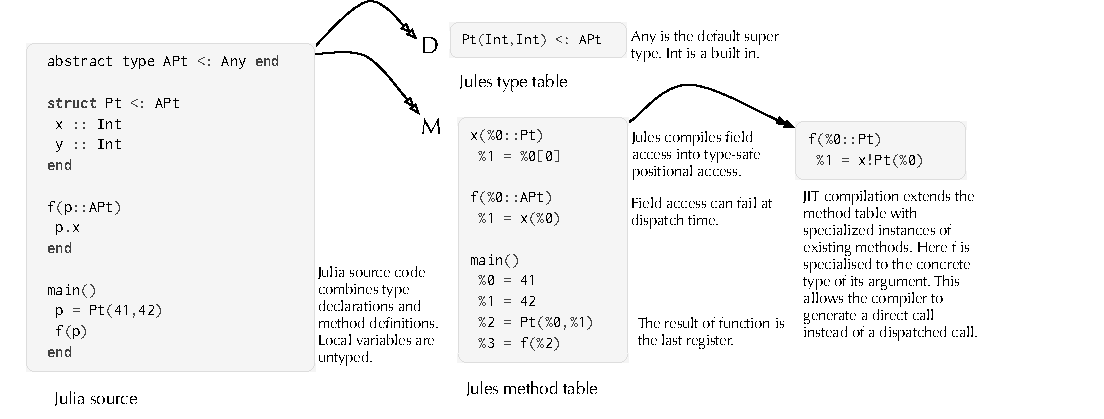
\includegraphics[width=1.1\columnwidth]{figs/compile.pdf}
  \caption{Compilation from Julia to \jules}\label{comp}
  \Description{Julia source code translated to Jules; one function is further compiled
    to a specialized version.}
\end{figure}

Fig.~\ref{comp} illustrates the relationship between Julia source code, the
\jules intermediate representation, and the result of compilation. We do not model
the translation from the source to \jules, and simply assume that the front-end
generates well-formed \jules code.\footnote{The front-end does not devirtualize
function calls, as Julia programmers do not have the ability to write direct
method invocations in the source.} A \jules program consists of an immutable \emph{type
table}~\tytbl and a \emph{method table}~\mtbl; the method table can be incrementally extended
with method instances that are compiled by the just-in-time compiler.

The source program of Fig.~\ref{comp} defines two types, the concrete \c{Pt} and
its parent, the abstract type \c{APt}, as well as two methods, \c{f} and
\c{main}. When translated to \jules, \c{Pt} is added to the type table along
with its supertype \c{APt}. Similarly, the methods \c{main} and \c{f} are added
to the \jules method table, along with accessors for the fields of \c{Pt}, with
bodies translated to the \jules intermediate representation.

The \jules IR is similar to static single assignment form. Each statement can
access values in registers, and saves its result into a new, consecutively
numbered, register. Statements can perform a dispatched call \c{f(\%2)}, direct
call \c{x\!Pt(\%0)}, conditional assignment (not shown), and a number of other
operations. The IR is untyped, but the translation from Julia is type sound. In
particular, type soundness guarantees that only dispatch errors can occur at run
time. For example, compilation will produce only well-formed field accesses such
as the one in \c{x(\%0::Pt)}, but a dispatched call \c{x(\%0)} in \c{f} could
fail if \c{f} was called with a struct that did not have an \c{x} field. In
order to perform this translation, \jules uses type inference to determine the
types of the program's registers. We abstract over this type inference mechanism
and only specify that it produces sound (with respect to our dynamic semantics)
results. %, but do not describe its operation.

Execution in \jules occurs between \emph{configurations} consisting of both
a stack of \emph{frames} \frm (representing the current execution state)
and a \emph{method table} \mtbl (consisting of original methods and specialized
instances), denoted $\config{\frm}{\mtbl}$. A configuration
$\config{\frm}{\mtbl}$ evolves to a new configuration
$\config{\frm'}{\mtbl'}$ by stepping $\config\frm\mtbl \step
\config{\frm'}{\mtbl'}$; every step processes the top instruction in $\frm$
and possibly compiles new method instances into $\mtbl'$. Notably, due to the
so-called world-age mechanism~\cite{oopsla20a} which restricts the effect
of \c{eval}, source methods are fixed from the
perspective of compilation; only compiled instances changes.

\section{Syntax}

The syntax of \jules methods is defined in~\figref{syntax}. We use two key
notational devices. First, sequences are denoted \ol{\,\cdot\,}; thus, \ol\ty
stands for types $\ty_0\dots\ty_n$, \ol{\v\k} for registers $\v\k_0\dots\v\k_n$,
and \ol\st for instructions $\st_0\dots\st_n$. An empty sequence is written
\emp. Second, indexing is denoted $[\cdot]$; \idx{\ol\ty}\k is the $k$-th type
in \ol\ty (starting from 0), \get\j\k is the $k$-th field of \v\j, and
\idx\mtbl{\msig\m{\ol\ty}} indexes \mtbl by method signature where \m denotes
method name and \ol\ty denotes argument types.

\begin{figure}[!h]\small
\begin{tabular}{llll}
\ty &::=& & type \\
    & | & \Ty  & \itshape concrete type \\
    & | & \aty & \itshape abstract type \\
\\
\tytbl &::=&  & type table \\
&&      $\left(\ \ \msig\Ty{\ol\ty} ~<:~ \aty \ \ \right)\!*$&\\
\mtbl&::=&  & {method table}\\
&&
  $\left(\ \ \langle \meth\m{\ol{\ty'}}{\ol{\v\j}}\ol\st,\ \ol{\ty}\rangle \ \ \right)\!*$\\
%\end{tabular}
%
%\begin{tabular}{ll@{~}ll}
\st &::=& & instruction\\
    & | & $\ass\i\p$ &\itshape int. assignment\\
    & | & $\ass\i{\v\j}$ &\itshape reg. transfer\\
    & | & $\ass\i{\construct\Ty{\ol{\v\k}}}$ & \itshape allocation\\
    & | & $\ass\i{\get\j\k}$ & \itshape field access\\
    & | & $\cond\i\j{\call\m{\ol{\v\k}}}{\v\l}$&\itshape dispatched call\\
    & | & $\cond\i\j{\direct\m{\ol{\Ty}}{\ol{\v\k}}}{\v\l}$&\itshape direct call\\
\multicolumn{3}{l}{$i \in \mathbb{N},\ \p \in \mathbb{Z}$} & \\
\end{tabular}
\caption{Syntax of \jules}\label{syntax}
\Description{Syntax of Jules}
\end{figure}

Types \ty live in the immutable type table \tytbl, which contains both concrete
(\Ty) and abstract (\aty) types. Each type table entry is of the form
$\msig{\Ty}{\ol\ty} <: \aty$, introducing concrete type $\Ty$, with fields of
types $\ol\ty$, along with the single supertype $\aty$. Two predefined types are
the concrete integer type \int, and the universal abstract supertype \any.

Method tables \mtbl contain method definitions of two sorts:
first, original methods that come from source code;
second, method instances compiled from original methods.
To distinguish between the two sorts, we store the type signature of the
original method in every table entry.
Thus, table entry
$\langle\meth\m{\ol{\ty'}}{\ol{\v\j}}\ol\st,\ \ol{\ty}\rangle$ describes a
method \m with parameter types $\ol{\ty'}$ and the body comprised of
instructions $\ol\st$; type signature \ol{\ty} points to the original method.
If \ol\ty is equal to \ol{\ty'}, the entry defines an original method,
and \ol{\st} cannot contain direct calls.%
\footnote{All function calls in Julia source code are dispatched calls.}
Otherwise, \ol{\ty'}
denotes some concrete types~\ol\Ty, and the entry defines a
method instance compiled from \msig\m{\ol\ty}, specialized for concrete argument
types $\ol\Ty <: \ol\ty$.
Method table may contain multiple method definitions with the same name,
but they have to have distinct type signatures.

Method bodies consist of instructions \ol{\st}. An instruction $\v{\i}
\leftarrow \text{\c{op}}$ consists of an operation \c{op} whose result is
assigned to register $\v\i$. An instruction can assign from a primitive integer
\p, another register \v\j, a newly created struct $\construct\Ty{\ol{\v\k}}$
of type \Ty with field values $\ol{\v\k}$, or the result of looking up a struct
field as $\get\j\k$. Finally, the instruction may perform a function call. Calls
can be dispatched, $\call\m{\ol{\v\k}}$, where the target method is dynamically
looked up, or they can be direct, \direct\m{\ol\Ty}{\ol{\v\k}}, where the target
method is specified. All calls are conditional: \EM{\v\j ~?~ \text{\c{call}} :
  \v\l}, to allow for recursive functions.
If the register \v\j is non-zero, then \c{call} is performed. Otherwise,
the result is the value of register \v\l. Conditional calls can be trivially
transformed into unconditional calls; in examples, this transformation is
performed implicitly.

\section{Dynamic Semantics}

\jules is parameterized over three components: method dispatch $\mathcal D$,
type inference $\mathcal I$, and just-in-time compilation \jit. We do not
specify how the first two work, and merely provide their interface and a set of
criteria that they must meet (in sections \ref{sec:disp} and \ref{sec:infer},
respectively). The compiler, \jit, is instantiated with either the identity
function, which gives a regular non-optimizing semantics, or an optimizing
compiler, which is defined in section~\ref{sec:comp}. The optimizing compiler
relies on type inference $\mathcal I$ to devirtualize method calls. Type
inference also ensures well-formedness of method tables. Method dispatch
$\mathcal D$ is used in operational semantics.

\begin{figure}[!t]\small
\begin{tabular}{rclcrclcrcl}
\val &::=& \p\ |\ \construct\Ty{\ol\val}
& \qquad &
\env &::=& \ol\val
& \qquad &
\frm &::=& \done\ |\ \stk{\env\ \ol\st}{\frm} \\
\end{tabular}
\begin{mathpar}
\PAPERVERSIONINLINE{}{\framebox{\configd \step \config{\frm'}{\mtbl}}\\}

\inferrule[Prim]{
  \st = \ass\i\p\\\\
  \env' = \env + \p
}{
  \config{ \stk{ \env \ \st\,\ol\st}{\frm} }{\mtbl} \step
  \config{ \stk{ \env'\ \ol\st     }{\frm} }{\mtbl}
}

\inferrule[Reg]{
  \st = \ass\i{\v\j}\\\\
   \env'=\env + \idx\env\j
}{
  \config{ \stk{ \env \ \st\,\ol\st}{\frm} }{\mtbl} \step
  \config{ \stk{ \env'\ \ol\st     }{\frm} }{\mtbl}
}

\inferrule[New]{
  \st= \ass\i{\construct\Ty{\ol{\v\k}}}\\\\
  \env'  = \env + \construct\Ty{\idx\env{\ol{k}}}
}{
  \config{ \stk{ \env \ \st\,\ol\st }{\frm} }{\mtbl} \step
  \config{ \stk{ \env'\ \ol\st      }{\frm} }{\mtbl}
}
\\

\inferrule[Field]{
  \st= \ass\i{\get\j\k}\\\\
  \val = \idx\env\j \and
  \env' = \env + \idx\val\k
}{
  \config{ \stk{ \env \ \st\,\ol\st }{\frm} }{\mtbl} \step
  \config{ \stk{ \env'\ \ol\st      }{\frm} }{\mtbl}
}

\inferrule[False1]{
  \st= \cond\i\j{\call\m{\ol{\v k}}}{\v\l}\\\\
  0 = \idx\env\j \and
  \env'=\env +  \idx\env\l
}{
  \config{ \stk{ \env \ \st\,\ol\st }{\frm} }{\mtbl} \step
  \config{ \stk{ \env'\ \ol\st      }{\frm} }{\mtbl}
}

\inferrule[False2]{
  \st= \cond\i\j{\direct\m{\ol\Ty}{\ol{\v\k}}}{\v\l}\\\\
  0 = \idx\env\j \and
  \env'=\env + \idx\env\l
}{
  \config{ \stk{ \env \ \st\,\ol\st }{\frm} }{\mtbl} \step
  \config{ \stk{ \env'\ \ol\st      }{\frm} }{\mtbl}
}
\\

\inferrule[Disp]{
  \st= \cond\i\j{\call\m{\ol{\v\k}}}{\v\l}\\\\
  0 \not=\idx\env\j \and
  \ol\Ty = \typeof(\idx\env{\ol{k}}) \and
  \mtbl' = \jit(\mtbl, \m, \ol\Ty) \\\\\
  \ol{\st'} = \body(\dispatch{\mtbl'}\m{\ol\Ty}) \and
  \env' =  \idx\env{\ol{k}}
}{
  \config{                        \stk{\env\ \st\,\ol\st}{\frm}  }{\mtbl} \step
  \config{ \env'\ \stk{\ol{\st'}}{\stk{\env\ \st\,\ol\st}{\frm}} }{\mtbl'}
}

\inferrule[Direct]{
  \st= \cond\i\j{\direct\m{\ol\Ty}{\ol{\v\k}}}{\v\l}\\\\
  0 \not = \idx\env\j \\\\
  \ol{\st'} = \body(\mtbl[\msig\m{\ol\Ty}]) \and
  \env' = \idx\env{\ol{k}}
}{
  \config{                        \stk{\env\ \st\,\ol\st}{\frm}  }{\mtbl} \step
  \config{ \env'\ \stk{\ol{\st'}}{\stk{\env\ \st\,\ol\st}{\frm}} }{\mtbl}
}

\inferrule[Ret]{
  \env''=\env + \last{\env'}
}{
  \config{ \stk{\env'\ \done}{\stk{ \env  \ \st\,\ol\st }{\frm}}}{\mtbl} \step
  \config{                    \stk{ \env''\ \ol\st      }{\frm} }{\mtbl}
}
\end{mathpar}
\caption{Dynamic semantics of Jules}\label{sems}
\Description{Dynamic semantics of Jules}
\end{figure}

\subsection{Operational Semantics}\label{sec:opsem}

Fig.~\ref{sems} gives rules for the dynamic semantics. Given a type table \tytbl
as context, \jules can step a configuration $\config{\frm}{\mtbl}$ to
$\config{\frm'}{\mtbl'}$, written as $\config\frm\mtbl \step
\config{\frm'}{\mtbl'}$.
Stack frames \frm consist of a sequence of environment-instruction list pairs.
Thus, $\stk{\env\ \ol\st}\frm$ denotes a stack with environment \env and
instructions \ol\st on top, followed by a sequence of environment-instruction
pairs. Each environment is a list of values $\env=\ol\val$, representing
contents of the sequentially numbered registers. Environments can then be
extended as $\env + \val$, indexed as $\idx\env\k$, and their last value is
\last\env if \env is not empty.

The small-step dynamic semantics is largely straightforward. The first four
rules deal with register assignment: updating the environment with a constant
value (\SC{Prim}), the value in another register (\SC{Reg}),
a newly constructed struct (\SC{New}), or the value in a field (\SC{Field}).
The remaining five rules deal with function calls, either dispatched
\call\m{\ol{\v\k}} or direct \direct\m{\ol\Ty}{\ol{\v\k}}.
Call instructions are combined with conditioning: a call can only be made after
testing the register \v\j, called a guard register.
If the register value is zero, then the value of the alternate register
\v\l is returned (\SC{False1/False2}).
Otherwise, the call can proceed, by \SC{Disp} for dispatched calls and \SC{Direct}
for direct ones.
%
A dispatched call starts by prompting the JIT compiler to
specialize method \m from the method table~\mtbl with the argument types \ol\Ty
and produce a new method table $\mtbl'$.
Next, using the new table $\mtbl'$, the dispatch mechanism $\mathcal D$
determines the method to invoke. Finally, the body \ol{\st'} of the method and
call arguments \idx\env{\ol{k}} form a new stack frame for the callee,
and the program steps with the extended stack and the new table.
%
Direct calls are simpler because
a direct call $\msig\m{\ol\Ty}$ uniquely identifies the
method to invoke. Thus, the method's instructions are looked up in \mtbl
by the method signature, a new stack frame is created,
and the program steps with the new stack and the same method table.
%
The top frame without instructions to execute indicates the
end of a function call (\SC{Ret}): the last value of the top-frame environment
becomes the return value of the call, and the top frame is popped from the stack.

Program execution begins with the frame $\emp\ \main()$%
\footnote{Recall that unconditional calls are implicitly expanded into conditional ones.},
i.e. a call to the \main function with an empty environment;
the execution either diverges, finishes with a final configuration $\env\ \done$,
or runs into an error.
We define two notions of error. An \emph{err} occurs only in the \SC{Disp} rule,
when the dispatch function $\mathcal D$ is undefined for the call; the \emph{err}
corresponds to a dynamic-dispatch error in Julia. A configuration is
\emph{wrong} if it cannot make a step for any other reason.
%the program is ill-formed. while \emph{erred} states are merely ill-typed.
%JB: we don't define a type system, so I would not use "ill-typed" terminology

\begin{definition}[Errors] A non-empty configuration \frm, \mtbl
 that cannot step $\frm, \mtbl \step \frm', \mtbl'$ has \emph{erred} if its
 top-most frame, \E\ \ol\st, starts with $\cond\i\j{\call\m{\ol{\v\k}}}{\v\l}$,
 where \ol\Ty is the types of \ol{\v\k} in \E, $\m\in\mtbl$, and
 \dispatch\mtbl\m{\ol\Ty} is undefined. Otherwise, \frm, \mtbl is
 \emph{wrong}.
\end{definition}

\subsection{Dispatch}\label{sec:disp}

\jules is parametric over method dispatch: any mechanism $\mathcal D$ that
satisfies the \emph{Dispatch Contract} (\defref{disprel}) can be used. Julia's
method dispatch mechanism
%is designed to, given a set of \emph{applicable} methods, return the \emph{most
%specific} one, if such method exists and is \emph{unique}. First, applicable
%JB: dispatch is not given applicable methods
is designed to, given method table, method name, and argument types,
return the \emph{most specific method applicable} to the given arguments
if such a method exists and is unique. First, applicable
methods are those whose declared type signature is a supertype of the argument
type. Then, the most specific method is the one whose type signature is the
most precise. Finally, only one most specific applicable method may exist, or
else an error is produced. Each of these components appears in our dispatch
definition. As in Julia, dispatch is only defined for tuples of concrete types.

\begin{definition}[Dispatch Contract] The \emph{dispatch} function
  $\dispatch\mtbl\m{\ol\Ty}$ takes method table \mtbl, method name \m,
  and concrete argument types \ol\Ty, and returns a method
  $\meth\m{\ol{\ty}}{\ol{\v\j}}\ol\st \in \mtbl$ such that
  the following holds (we write $\ol\ty <: \ol{\ty'}$ as a shorthand for
  $\forall i.\,\ty_i<:\ty'_i$):
  \begin{enumerate}
    \item $\ol\Ty <: \ol\ty$, meaning that $\msig\m{\ol\ty}$
      is applicable to the given arguments;
    \item $\forall \meth\m{\ol{\ty'}}{\ol{\v\j}}\ol\st \in \mtbl.\ \
      \ol\Ty <: \ol{\ty'}\ \implies\ \ol{\ty} <: \ol{\ty'},$
      meaning that $\msig\m{\ol\ty}$ is the most specific applicable method.
  \end{enumerate}
  \label{disprel}
\end{definition}

\subsection{Inference}\label{sec:infer}

The Julia compiler infers types of variables by forward data-flow analysis. Like
dispatch, inference is complex, so we parameterize over it. For our purposes, an
inference algorithm~$\mathcal I$ returns a sound typing for a sequence of
instructions in a given method table,
$\typeinf{\origmtbl{\mtbl}}{\ol\ty}{\ol\st}=\ol{\ty'}$, where \origmtbl{\mtbl}
denotes the table containing only methods without direct calls. Inference
returns types $\ol\ty'$ such that each $\ty'_i$ is the type of register of
$\st_i$. Any inference algorithm that satisfies the \SC{Soundness} and
\SC{Monotonicity} requirements is acceptable.

\begin{requirement}[Soundness] If
  $\typeinf\mtbl{\ol\ty}{\ol\st} = \ol{\ty'}$, then
  for any environment \env compatible with \ol\ty, that is, $\typeof(E_{i}) <: \ty_{i}$,
  and for any stack $\frm$, the following holds:
%
  \begin{enumerate}
  \item If
  $\config{\stk{\env\ \ol\st}\frm}{\mtbl} \stepmul \stk{\frm'}{\frm},\mtbl'$
  and %$\stk{\frm'}{\frm},\mtbl'$
  cannot make another step,
  then $\stk{\frm'}{\frm},\mtbl'$ has \emph{erred}.
  %
  \item If $\config{\stk{\env\ \ol\st}{\frm}}{\mtbl} \stepmul
    \config{\stk{\env\,\env'\ \ol{\st''}}{\frm}}{\mtbl'}$,
  then $\ol\st = \ol{\st'}\,\ol{\st''}$ and $\typeof(\env'_{i}) <: \ty'_{i}$.
  \end{enumerate}
  % In particular,
  % \item $\config{\stk{\env\ \ol\st}{\frm}}{\mtbl} \stepmul
  %   \config{\stk{\env\,\env'\ \done}{\frm}}{\mtbl'}$
  % where $\typeof(\env') <: \ol{\ty'}$, or
 \end{requirement}

The soundness requirement guarantees that if type inference succeeds on a method,
then, when the method is called with compatible arguments,
it will not enter a \emph{wrong} state but may \emph{err} at a dynamic call.
Furthermore, if the method terminates, all its instructions evaluate
to values compatible with the results of type inference.
That is, when $\config{\stk{\env\ \ol\st}{\frm}}{\mtbl} \stepmul
\config{\stk{\env\,\env'\ \done}{\frm}}{\mtbl'}$, we have
$\typeof(\env') <: \ol{\ty'}$.

The second requirement of type inference, monotonicity, is important to specialization:
it guarantees that using more precise argument types for original method
bodies succeeds and does not break assumptions of the caller about
the callee's return type. If inference was not
monotonic, then given more precise argument types, it could return
a method specialization with a less precise return type. As a result,
translating a dynamically dispatched call into a direct call may be unsound.

\begin{requirement}[Monotonicity]\label{prop:ti-monot}
  For all $\mtbl, \ol{\ty},
  \ol\st, \ol{\ty'},$ such that $\typeinf\mtbl{\ol{\ty}}{\ol\st} = \ol{\ty'}$,
  \[
    \forall\, \ol{\ty''}.\quad \ol{\ty''} <: \ol{\ty}
    \quad \implies \quad
    \exists \ol{\ty'''}.\ \
    \typeinf\mtbl{\ol{\ty''}}{\ol\st} = \ol{\ty'''} \ \ \land\ \
    \ol{\ty'''} <: \ol{\ty'}.
  \]
\end{requirement}

\subsection{Well-Formedness}\label{wellform}

Initial \jules configuration \config{\emp\ \main()}{\mtbl} is well-formed
if the method table \mtbl is well-formed according to \defref{ref:def-well-formed}.
Such a configuration will either successfully terminate, \emph{err},
or run forever, but it will never reach a \emph{wrong} state.
%We can now define what it means for a \jules program to be well-formed.
%: \TODO{we then defined well-formed table; make sure it's clear what a program is}

\begin{definition}[Well-Formedness of Method Table]\label{ref:def-well-formed}
A method table is \emph{well-formed} $\mathit{WF}(\mtbl)$ if the following
holds:
\begin{enumerate}
\item Entry method $\msig{\SF{main}}\emp$ belongs to $\mtbl$.
\item Every type \ty in \mtbl, except \int and \any, is declared in \tytbl.
\item Registers are numbered consecutively from 0, increasing by one for each
  parameter and instruction. An instruction assigning to \v\k only refers to
  registers \v\i such that $i<k$.
\item For any original method $\langle
  \meth\m{\ol{\ty}}{\ol{\v\j}}\ol\st,\ \ol\ty \rangle \in \mtbl$, the body is
  not empty and does not contain direct calls, and type
  inference succeeds
  $\typeinf{\origmtbl{\mtbl}}{\ol\ty}{\ol\st}=\ol{\ty'}$
  on original methods \origmtbl\mtbl.
\item Any two methods in \mtbl with the same name,
  $\msig{\m}{\ol\ty}$ and $\msig{\m}{\ol{\ty'}}$, have distinct type
  signatures, i.e. $\ol\ty \neq \ol{\ty'}$.
  \item For any method specialization $\langle \msig\m{\ol{\ty'}}, \ol{\ty}\rangle\in\mtbl$,
  i.\,e. $\ol{\ty'} \neq \ol{\ty}$, the following holds:
  $\ol{\ty'} = \ol\Ty$, and
  $\ol{\Ty} <: \ol{\ty}$, and
  $\langle \msig\m{\ol{\ty}}, \ol{\ty}\rangle\in\mtbl$.
  Moreover,
   $\forall \msig\m{\ol\ty''} \in \mtbl.\
      \ol\Ty <: \ol{\ty''} \implies \ol{\ty} <: \ol{\ty''}$.
\end{enumerate}
\end{definition}

The last requirement ensures that only the most specific original methods have
specializations, which precludes compilation from modifying program behavior.
%
For example, consider type hierarchy
\c{Int<:Number<:Any} and function \c{f} with original methods for \c{Any} and
\c{Number}. If there are no compiled method instances, the call \c{f(5)}
dispatches to \c{f(::Number)}. But if the method table contained a specialized
instance \c{f(::Int)} of the original method \c{f(::Any)}, the call would dispatch
to that instance, which is not related to the originally used \c{f(::Number)}.
Thus, program behavior would be modified by compilation, which is undesired.

\begin{figure}[!t] \small\begin{mathpar}
\Rule{CompileTrue}{
  \msig{\m}{\ol\Ty} \not\in \mtbl \and
  \ol\st = \body(\dispatch\mtbl\m{\ol\Ty}) \and
  \ol{\ty'} = \typeinf{\origmtbl{\mtbl}}{\ol\Ty}{\ol\st}
  \\
  \ol{\ty} = \mathit{signature}(\dispatch\mtbl\m{\ol\Ty}) \and
  \mtbl_0 = \mtbl + \langle \msig\m{\ol{\Ty}}\done, \ol\ty \rangle
  \\
  \ol\Ty\,\ol{\ty'} \vdash \st_0, \mtbl_0 \leadsto \st'_0,\mtbl_1\and
  \dots\and
  \ol\Ty\,\ol{\ty'} \vdash \st_n, \mtbl_n \leadsto  \st'_n,\mtbl_{n+1} \\
  \mtbl' = \mtbl_{n+1} [\msig\m{\ol{\Ty}} \mapsto \langle \meth\m{\ol\Ty}{\ol{\v k}} \ol{\st'},\ol{\ty}\rangle]
}{% \mapsto \langle \meth\m{\ol\Ty}{\ol{\v k}} \ol{\st'},\ol{\ty}
   \jit(\mtbl,\m,\ol\Ty) = \mtbl'
}

\Rule{CompileFalse}{
  \msig{\m}{\ol\Ty} \in \mtbl
}{
  \jit(\mtbl,\m,\ol\Ty) = \mtbl
}

\Rule{Dispatch}{
  \st = \cond\i\j{\call\m{\ol{\v\k}}}{\v\l} \and
  \ol{\Ty} = \ol\ty[\ol\k] \\\\
  \mtbl' = \jit(\mtbl,\m,\ol{\Ty}) \and
  \st' = \cond\i\j{\direct\m{\ol{\Ty}}{\ol{\v\k}}}{\v\l}
}{
  \ol\ty\ \vdash\ \st,\mtbl \leadsto \st',\mtbl'
}

\Rule{NoDispatch}{
  \st \neq \cond\i\j{\call\m{\ol{\v\k}}}{\v\l}\\\\
  \text{or} \and
  \ol{\Ty} \neq \ol\ty[\ol\k]
}{
  \ol\ty\ \vdash\ \st,\mtbl \leadsto \st,\mtbl
}
\end{mathpar}

  \caption{\MODIFY{Compilation: extending method table with a specialized method
  instance (top rule) and replacing a~dynamically dispatched call with
  a direct method invocation in the extended table (bottom-right)}}\label{compile}
\Description{Compilation: extending method table with a specialized method
  instance and replacing a~dynamically dispatched call with
  a direct method invocation in the extended table}
\end{figure}

\subsection{Compilation}\label{sec:comp}

\jules implements devirtualization through the $\jit(\mtbl,\m,\ol\Ty)$
operation, shown in \figref{compile}. The compiler specializes methods according to the
inferred type information, replacing non-\emph{err} dispatched calls with direct calls where
possible. Compilation begins with some bookkeeping. First, it ensures that there
is no pre-existing instance in the method table before compiling;
otherwise, the table is returned immediately without modification, by
the bottom-left rule. Next, using dispatch,
it fetches the most applicable original method to compile. Then, using concrete argument types,
the compiler runs the type inferencer on the method's body, producing an
instruction typing \ol{\ty'}. Because the original method table is well-formed,
monotonicity of $\mathcal I$ and the definition of $\mathcal D$ guarantee that
type inference succeeds for $\ol\Ty <: \ol\ty$. Lastly, the compiler can begin
translating instructions. Each instruction $\st_i$ is translated into an
optimized instruction $\st'_i$. This translation respects the existing type
environment containing the argument types \ol\Ty and instruction typing
$\ol{\ty'}$. The translation $ \ol\ty\ \vdash\ \st,\mtbl \leadsto \st',\mtbl'$
leaves all instructions unchanged except dispatched calls. Dispatched calls
cause a recursive JIT invocation, followed by rewriting to a direct call. To
avoid recursive compilation, a stub method $\langle \msig\m{\ol{\Ty}}\done,
\ol\ty \rangle$ is added at the beginning of compilation,
and over-written when compilation is done. As the source program is finite and
new types are not added during compilation, it terminates. Note that if
the original method has concrete argument types, the compiler does nothing.


\section{Type Groundedness and Stability}\label{sec:stability-formal}
%%------------------------------

We now formally define the properties of interest, type stability and type
groundedness. Recall the informal definition which stated that a function is
type stable if its return type depends only on its argument types, and type grounded
if every variable's type depends only on the argument types. In this
definition, ``types'' really mean concrete types, as concrete types allow for
optimizations. The following defines what it means for an original method to be
type stable and type grounded.

\begin{definition}[Stable and Grounded]\label{def:ground}
  Let \meth{\m}{\ol\ty}{}{\ol\st} be an original method in a well-formed
  method table \mtbl. Given concrete argument types $\ol\Ty <: \ol\ty$,
  if $\typeinf{\origmtbl{\mtbl}}{\m}{\ol\Ty} = \ol{\ty'}$,
  and
  \begin{enumerate}
  \item  $\last{\ol{\ty'}} = \Ty'$, i.e. the return type is concrete, then
    the method is \emph{type stable for \ol\Ty},
  \item $\ol{\ty'} = \ol{\Ty'}$, i.e. all register types are concrete, then the
    method is \emph{type-grounded for \ol\Ty}.
  \end{enumerate}

  Furthermore, a method is called \emph{type stable (grounded) for a set $W$
  of concrete argument types} if it is type stable (grounded) for every
  $\ol\Ty \in W$.
\end{definition}

As all method instances are compiled from some original method definitions,
type stabiltiy and groundedness for instances is defined in terms of their
originals.

\begin{definition}\label{def:ground-inst}
  A method instance $\langle \meth{\m}{\ol\Ty}{}{\ol{\st'}},\ \ol\ty \rangle$
  is called \emph{type stable (grounded)},
  if its original method \msig\m{\ol\ty} is type stable (grounded) for \ol\Ty.
\end{definition}


\subsection{Full Devirtualization}\label{sec:ground-inst-prop}

The key property of type groundedness is that
compiling a type-grounded method results in a fully devirtualized instance.
We say that a method instance \meth\m{\ol\Ty}{\ol{\v k}}\ol{\st} is \emph{fully devirtualized}
if \ol{\st} does not contain any dispatched calls. To show that \jit
indeed has the above property, we will need an additional
notion, \emph{maximal devirtualization}, which is defined
in~\figref{fig:max-devirt}. Intuitively, the predicate \devirtst{\ol\ty}{\mtbl}{\st}
states that an instruction \st does not contain a dispatched call
that can be resolved in table \mtbl for argument types found in \ol\ty.
Then, a method instance is maximally devirtualized if this predicate
holds for every instruction using \ol\ty that combines argument types with
the results of type inference.

\begin{figure}[!t]\small
\begin{mathpar}
%
\PAPERVERSIONINLINE{\\}{\framebox{\devirtst{\ol\ty}{\mtbl}{\st}}\\}%

\inferrule[D-NoCall]{
  \st \neq \cond\i\j{\call\m{\ol{\v\k}}}{\v\l} \and
  \st \neq \cond\i\j{\call{\msig\m{\ol{\Ty}}}{\ol{\v\k}}}{\v\l}
}{
  \devirtst{\ol\ty}{\mtbl}{\st}
}
\\

\inferrule[D-Disp]{
  \st = \cond\i\j{\call\m{\ol{\v\k}}}{\v\l} \and
  \ol\Ty \neq \idx{\ol\ty}{\ol\k}
}{
  \devirtst{\ol\ty}{\mtbl}{\st}
}

\inferrule[D-Direct]{
  \st = \cond\i\j{\call{\msig\m{\ol\Ty}}{\ol{\v\k}}}{\v\l} \and
  \ol\Ty = \idx{\ol\ty}{\ol\k} \and
  \msig{\m}{\ol{\Ty}} \in \mtbl
}{
  \devirtst{\ol\ty}{\mtbl}{\st}
}
\\

\PAPERVERSIONINLINE{}{\framebox{\devirtst{\ol\ty}{\mtbl}{\ol\st}}\\}
%
\inferrule[D-Seq]{
  \devirtst{\ol\ty}{\mtbl}{\st_0} \and \ldots \and
  \devirtst{\ol\ty}{\mtbl}{\st_n}
}{
  \devirtst{\ol\ty}{\mtbl}{\ol\st}
}
\\

\PAPERVERSIONINLINE{}{\framebox{\devirtm{\mtbl}}\\}%
%
\inferrule[D-Table]{
  \forall \langle \meth\m{\ol\Ty}{}\ol{\st'},\ol{\ty} \rangle \in \mtbl. \ \ \
  \ol\Ty \neq \ol\ty \ \land\ \ol{\st'} \neq \done \ \ \ \implies \ \ \
  \meth\m{\ol\ty}{}\ol{\st} \in \mtbl \ \ \land \ \
  \ol{\ty'} = \typeinf{\origmtbl{\mtbl}}{\ol\Ty}{\ol\st} \ \ \land \ \
  \devirtst{\ol\Ty\,\ol{\ty'}}{\mtbl}{\ol{\st'}}
}{
  \devirtm{\mtbl}
}
\end{mathpar}
\caption{\MODIFY{Maximal devirtualization of instructions
  and method tables}}\label{fig:max-devirt}
\Description{Maximal devirtualization of instructions
  and method tables}
\end{figure}


Next, we review the definition from~\figref{fig:max-devirt} in more details.
\SC{D-NoCall} states that an instruction without a call
is maximally devirtualized. \SC{D-Disp} requires that for a dispatched call,
\ol\ty does not have precise enough type information to resolve the call with
$\mathcal{D}$. Finally, \SC{D-Direct} allows a direct call to a concrete method
with the right type signature: as concrete types do not have subtypes, the
\msig\m{\ol\Ty} with concrete argument types is exactly the definition that a call
\call\m{\ol{\v\k}} would dispatch to. \SC{D-Seq} simply checks that all
instructions in a sequence \ol\st are devirtualized in the same register typing
\ol\ty. Here, \ol\ty has to contain typing for all instructions $\st_i$, because
later instructions refer to the registers of the previous ones. The last rule
\devirtm{\mtbl} covers the entire table \mtbl, requiring all methods to be maximally
devirtualized. Namely, \SC{D-Table} says that for all method instances
(condition $\ol\Ty \neq \ol\ty$ implies that \msig\m{\ol\Ty}
is not an original method) that are not
stubs ($\ol{\st'} \neq \done$), the body \ol{\st'} is maximally devirtualized
according to the typing of the original method with respect to the instance's
argument types.

Using the notion of maximal devirtualization, we can connect type groundedness
and full devirtualization.

\begin{lemma}[Full Devirtualization]\label{lem:full-virt}
  If \mtbl is well-formed and maximally devirtualized, then any type-grounded
  method instance $\meth\m{\ol\Ty}{\ol{\v k}}\ol{\st'} \in \mtbl$ is fully
  devirtualized.
\end{lemma}
\begin{proof}
\PAPERVERSION{
  Follows from the definitions of type groundedness and maximal
  devirtualization; details can be found in the extended
  version~\cite{oopsla21jules:arx}.
}{
  Recall that a method instance is type-grounded if type inference
  produces concrete typing \ol{\Ty'} for the original method body \ol\st, i.e.
  $\typeinf{\origmtbl{\mtbl}}{\ol\Ty}{\ol\st} = \ol{\Ty'}$.
  By the definition of a maximally devirtualized table, we know that
  \devirtst{\ol\Ty\,\ol{\Ty'}}{\mtbl}{\ol{\st'}}.
  Since all types in the register typing $\ol\Ty\,\ol{\Ty'}$ are concrete,
  by analyzing maximal devirtualization for instructions, we can see
  that the only applicable rules are \SC{D-NoCall} and \SC{D-Direct}.
  Therefore, \ol{\st'} does not contain any dispatched calls.
}
\end{proof}

\begin{figure}\small
\begin{mathpar}
\PAPERVERSIONINLINE{}{\framebox{\compst{\ol\ty}{\st}{\mtbl}{\S}{\st'}{\mtbl'}{\S'}}\\}

\inferrule[C-NoDisp]{
  \st \neq \cond\i\j{\call\m{\ol{\v\k}}}{\v\l}
}{
  \compst{\ol\ty}{\st}{\mtbl}{\S}{\st}{\mtbl}{\S}
}

\inferrule[C-Disp]{
  \st = \cond\i\j{\call\m{\ol{\v\k}}}{\v\l} \and
  \ol\Ty \neq \idx{\ol\ty}{\ol\k}
}{
  \compst{\ol\ty}{\st}{\mtbl}{\S}{\st}{\mtbl}{\S}
}

\inferrule[C-Direct]{
  \st = \cond\i\j{\call\m{\ol{\v\k}}}{\v\l} \and
  \ol\Ty = \idx{\ol\ty}{\ol\k} \and
  \msig{\m}{\ol\Ty} \in \mtbl \and
  \st' = \cond\i\j{\call{\msig\m{\ol\Ty}}{\ol{\v\k}}}{\v\l}
}{
  \compst{\ol\ty}{\st}{\mtbl}{\S}{\st'}{\mtbl}{\S}
}

\inferrule[C-Instance]{
  \st = \cond\i\j{\call\m{\ol{\v\k}}}{\v\l} \and
  \ol\Ty = \idx{\ol\ty}{\ol\k} \and
  \meth{\m}{\ol{\ty'}}{}{\ol\st} = \dispatch\mtbl\m{\ol\Ty} \and
  \ol\Ty \neq \ol{\ty'} \\\\
  \ol{\ty''} = \typeinf{\origmtbl{\mtbl}}{\ol\Ty}{\ol\st} \and
  \mtbl_0 = \mtbl + \langle \msig\m{\ol{\Ty}}\done, \ol{\ty'} \rangle \\\\
  \compst{\ol\Ty\,\ol{\ty''}}{\st_0}{\mtbl_0}{\S_0}{\st'_0}{\mtbl_1}{\S_1} \and
  \ldots \and
  \compst{\ol\Ty\,\ol{\ty''}}{\st_n}{\mtbl_n}{\S_n}{\st'_n}{\mtbl_{n+1}}{\S_{n+1}} \\\\
  \st' = \cond\i\j{\call{\msig\m{\ol\Ty}}{\ol{\v\k}}}{\v\l} \and
  \mtbl' = \mtbl_{n+1} + \langle \meth\m{\ol\Ty}{\ol{\v k}} \ol{\st'},\ol{\ty'} \rangle
}{
  \compst{\ol\ty}{\st}{\mtbl}{\S}{\st'}{\mtbl'}{\S'}
}
\end{mathpar}
\caption{Reformulated compilation}\label{fig:compile-wd}
\Description{Reformulated compilation}
\end{figure}

The final step is to show that compilation defined in \figref{compile} preserves
maximal devirtualization. To simplify the proof, \figref{fig:compile-wd}
reformulates \figref{compile} by inlining \jit into the compilation
relation. The relation does not have a rule for processing direct calls because
we compile only original methods. Since the set of method instances is finite,
the relation is well-defined: every recursive call to compilation happens
for a method table that contains at least one more instance.
Every compilation step produces a maximally devirtualized instruction and
potentially extends the method table with
new maximally devirtualized instances.

\MODIFY{

\begin{lemma}[Preserving Well Formedness]\label{lem:wf}
  For any method table \mtbl that is well-formed $\mathit{WF}(\mtbl)$,
  register typing \ol\ty, and instruction \st,
  if the instruction \st is compiled,
  $\compst{\ol\ty}{\st}{\mtbl}{\S}{\st'}{\mtbl'}{\S'},$
  then the new table is well-formed $\mathit{WF}(\mtbl')$.
\end{lemma}
\begin{proof}
  By induction on the derivation of
  \compst{\ol\ty}{\st}{\mtbl}{\S}{\st'}{\mtbl'}{\S'}.
  The only case that modifies the method table is \SC{C-Instance}.
\PAPERVERSION{
  There, by analyzing $\mtbl_0$, we can see that it is well-formed,
  and thus the induction hypothesis can be applied to
  \compst{\ol\Ty\,\ol{\ty''}}{\st_0}{\mtbl_0}{\S_0}{\st'_0}{\mtbl_1}{\S_1},
  and then to all
  \compst{\ol\Ty\,\ol{\ty''}}{\st_i}{\mtbl_i}{\S_0}{\st'_i}{\mtbl_{i+1}}{\S_{i+1}}.
  Since $\mtbl_{n+1}$ is well-formed, so is $\mtbl'$.
  More details are available in the extended version~\cite{oopsla21jules:arx}.
}{
  Let us analyze $\mtbl_0$ first.
  Since $\ol\Ty \neq \ol{\ty'}$ and \mtbl is well-formed,
  we know that \msig\m{\ol{\ty'}} is an original method and $\ol\Ty \neq \ol{\ty'}$.
  Furthermore, as dispatch is known to return the most applicable method,
  $\msig\m{\ol\Ty} \notin \mtbl$ and properties (5) and (6) of
  \defref{ref:def-well-formed} for $\mtbl_0$ are satisfied.
  Other properties are trivially satisfied because $\mtbl_0$
  does not add or modify any original methods, so:
  \[\mathit{WF}(\mtbl_0).\]
  Therefore, we can apply the induction hypothesis to
  \compst{\ol\Ty\,\ol{\ty''}}{\st_0}{\mtbl_0}{\S_0}{\st'_0}{\mtbl_1}{\S_1}
  to get $\mathit{WF}(\mtbl_1).$
  Proceeding in this manner, we arrive to:
  \[\mathit{WF}(\mtbl_{n+1}).\]
  As $\mtbl'$ only changes the body of the compiled instance \msig\m{\ol\Ty}
  compared to the well-formed $\mtbl_{n+1}$, we get the desired conclusion:
  \[\mathit{WF}(\mtbl').\]
}
\end{proof}

\begin{lemma}[Preserving Maximal Devirtualization]\label{lem:max-devirt}
  For any well-formed method table \mtbl, register typing \ol\ty,
  and instruction \st, if the method table is maximally devirtualized,
  \devirtm{\mtbl},  and the instruction \st is compiled,
  $\compst{\ol\ty}{\st}{\mtbl}{\S}{\st'}{\mtbl'}{\S'},$
  then the following holds:
  \begin{enumerate}
    \item the resulting instruction is maximally devirtualized in the new table,
      \devirtst{\ol\ty}{\mtbl'}{\ol{\st'}},
    \item the new table is maximally devirtualized, \devirtm{\mtbl'},
    \item any maximally devirtualized instruction stays maximally devirtualized
      in the new table,
      $\forall\, \ol{\ty^x}, \ol{\st^x}.\quad
      \devirtst{\ol{\ty^x}}{\mtbl }{\ol{\st^x}}\ \implies\
      \devirtst{\ol{\ty^x}}{\mtbl'}{\ol{\st^x}}$.
  \end{enumerate}
\end{lemma}

\begin{proof}
\PAPERVERSION{
  By induction on the derivation of
  \compst{\ol\ty}{\st}{\mtbl}{\S}{\st'}{\mtbl'}{\S'}.
  The most interesting case is \SC{C-Instance} where
  compilation of additional instances happens.
  The key step of the proof is to observe that the induction hypothesis
  is applicable to
  \compst{\ol\Ty\,\ol{\ty''}}{\st_0}{\mtbl_0}{\S_0}{\st'_0}{\mtbl_1}{\S_1},
  and then to all consecutive
  \compst{\ol\Ty\,\ol{\ty''}}{\st_i}{\mtbl_i}{\S_0}{\st'_i}{\mtbl_{i+1}}{\S_{i+1}},
  which is possible due to \lemref{lem:wf} and facts (2).
  Using facts (3), we propagate the information about maximal devirtualization
  of $\st_i$ in their respective tables to the final $\mtbl'$.
  A complete proof is available in~\cite{oopsla21jules:arx}.
}
{
  By induction on the derivation of
  \compst{\ol\ty}{\st}{\mtbl}{\S}{\st'}{\mtbl'}{\S'}.
  \begin{itemize}
    \item Cases \SC{C-NoDisp} and \SC{C-Disp} are straightforward:
      to show (1), we use rules \SC{D-NoCall} and \SC{D-Disp}, respectively.
      Since the resulting method table \mtbl is the same, (2) and (3)
      hold trivially.

    \item Case \SC{C-Direct}. By assumption, we know that
      $\ol\Ty = \idx{\ol\ty}{\ol\k}$ and that $\msig{\m}{\ol\Ty} \in \mtbl$.
      Therefore, we have (1) by \SC{D-Direct}:
      \[\devirtst{\ol\ty}{\mtbl}{\cond\i\j{\call{\msig\m{\ol\Ty}}{\ol{\v\k}}}{\v\l}}.\]
      The resulting method table \mtbl is the same, so (2) and (3) hold.

    \item Case \SC{C-Instance}. This is the interesting case where
      compilation of additional instances happens.
      First, note that $\mtbl_0$ is the same as \mtbl except for a new instance
      stub $\langle \msig\m{\ol{\Ty}}\done, \ol{\ty'} \rangle$.
      By assumption, \devirtm{\mtbl} holds, and \SC{D-Table} does not impose
      any constraints on stubs, so \devirtm{\mtbl_0} also holds.
      As shown in the proof of \lemref{lem:wf}, $\mtbl_0$ is also well-formed.
      Therefore, we can apply the induction hypothesis to
      \[\compst{\ol\Ty\,\ol{\ty''}}{\st_0}{\mtbl_0}{\S_0}{\st'_0}{\mtbl_1}{\S_1},\]
      and we get that:
      \begin{itemize}
        \item \devirtst{\ol\Ty\,\ol{\ty''}}{\mtbl_1}{\st'_0},
        \item \devirtm{\mtbl_1}, and
        \item $\forall\, \ol{\ty^x}, \ol{\st^x}.\quad
        \devirtst{\ol{\ty^x}}{\mtbl_0}{\ol{\st^x}}\ \implies\
        \devirtst{\ol{\ty^x}}{\mtbl_1}{\ol{\st^x}}$.
      \end{itemize}
      The fact that $\mtbl_1$ is maximally devirtualized by (2)
      and well-formed by \lemref{lem:wf}, lets us apply the
      induction hypothesis to the next instruction $\st_1$ of the method
      body \ol\st, and so on.  By repeating the same steps, we get
      that the final table obtained by compiling the body is
      also maximally devirtualized:
        \[\devirtm{\mtbl_{n+1}}.\]
      Now, let us look at the property (3) that we need to prove.
      Assuming we have some \ol{\ty^x}, \ol{\st^x} such that
      \devirtst{\ol{\ty^x}}{\mtbl }{\ol{\st^x}},
      we want to show that
      \devirtst{\ol{\ty^x}}{\mtbl'}{\ol{\st^x}}.
      First, observe that by case analysis on the derivation of
      \devirtst{\ol{\ty^x}}{\mtbl }{\ol{\st^x}},
      we can show that the property holds in $\mtbl_0$, i.e.
        \devirtst{\ol{\ty^x}}{\mtbl_0}{\ol{\st^x}}.
      For an instruction that is not a direct call, the presence of an additional
      method instance is irrelevant. If an instruction is a direct call to an
      existing method instance, it stays maximally devirtualized because
      $\mtbl_0$ does not remove or alter any existing instances of \mtbl.\\
      Next, we can apply the fact (3) from the induction on $\st_0$
      to conclude that \devirtst{\ol{\ty^x}}{\mtbl_1}{\ol{\st^x}},
      and so on, until we get that
        \[\devirtst{\ol{\ty^x}}{\mtbl_{n+1}}{\ol{\st^x}}.\]
      Since $\mtbl'$ only replaces the body of $\msig\m{\ol\Ty}$,
      by case analysis similar to the above, we conclude
        \[\devirtst{\ol{\ty^x}}{\mtbl'}{\ol{\st^x}},\]
      which \emph{proves (3)} for \SC{C-Instance}.
      Proceeding with similar reasoning, we can chain facts (3) from all
      intermediate compilations and apply them to facts (1) of the induction,
      so we get that
        \[\forall i.\quad \devirtst{\ol\Ty\,\ol{\ty''}}{\mtbl'}{\st'_i},\]
      and thus by \SC{D-Seq},
        \[\devirtst{\ol\Ty\,\ol{\ty''}}{\mtbl'}{\ol{\st'}}.\]
      Since the compilation does not remove or alter any original methods,
      $\origmtbl{\mtbl'} = \origmtbl{\mtbl}$, and thus
      type inference \typeinf{\origmtbl{\mtbl'}}{\ol\Ty}{\ol\st} produces
      the same results as \typeinf{\origmtbl{\mtbl}}{\ol\Ty}{\ol\st}.
      Therefore, the requirement of \SC{D-Table} for the method instance
      $\langle \meth\m{\ol\Ty}{\ol{\v k}}\ol{\st'},\ \ol{\ty'} \rangle$
      in $\mtbl'$ is satisfied to \emph{prove (2)}.\\
      Finally, we can \emph{prove (1)} for $\mtbl'$ by \SC{D-Direct}
      because $\msig\m{\ol\Ty} \in \mtbl'$.
  \end{itemize}
}
\end{proof}

%%%% JAN: If a method is fully devirtualized then of course it does not dispatch
%% JB: the theorem puts together the lemmas and the run-time semantics.
%%     Replaced by text for the main version.

Putting it all together, we have shown that type-grounded methods
compile to method instances without dynamically dispatched calls.
\PAPERVERSION{
Namely, since a well-formed original table
is trivially maximally devirtualized, and compilation preserves this property
by \lemref{lem:max-devirt},
executing a well-formed program results in a method table where
all method instances are maximally devirtualized. Furthermore, type-grounded
instances are fully devirtualized by \lemref{lem:full-virt},
and thus do not contain dispatched calls.
\begin{theorem}[Grounded Methods Never Dispatch]
  For any initial well-formed \mtbl, if
  \[ \config{\done\ \main()}{\mtbl} \stepmul
    \config{\stk{\env\ (\cond\i\j{\call{\msig\m{\ol\Ty}}{\ol{\v\k}}}{\v\l})\,\ol\st}{\frm}}{\mtbl'}
    \quad
    \wedge
    \quad
    \text{\msig{\m}{\ol\Ty} is type-grounded in $\mtbl'$,}
  \]
  then \msig{\m}{\ol\Ty} is fully devirtualized in $\mtbl'$.
\end{theorem}
}{
\begin{proof}
  First, observe that the initial table \mtbl is maximally devirtualized because
  it does not contain any compiled method instances. Then, by induction on
  \stepmul, we can show that the dynamic semantics preserves maximal
  devirtualization of the method table.
  Namely, by case analysis on one step of the dynamic semantics, we can see that the
  only rule that affects the method table is \SC{Disp}; all other rules simply
  propagate the same maximally devirtualized table.

  In the case of \SC{Disp}, by \lemref{lem:max-devirt},
  the new method table $\mtbl'$ is also maximally devirtualized.
  Since every step of the dynamic semantics preserves maximal devirtualization
  of the method table, so does the multi-step relation \stepmul.

  If the execution gets to a direct call, the call must have been produced
  by the JIT compiler.  As all compiled code is maximally devirtualized,
  by \SC{D-Direct}, the method instance \msig\m{\ol{\Ty}} exists,
  and, by \SC{D-Table}, it is known to be maximally devirtualized.
  Finally, as we know by \lemref{lem:full-virt}, any maximally devirtualized
  method instance that is type-grounded, is also fully devirtualized,
  and thus, it does not contain dispatched calls.
\end{proof}
}

}

\subsection{Relationship between Stability and Groundedness}\label{sec:stable}

\MODIFY{
While it is type groundedness that enables devirtualization,
the weaker property, type stability, is also important in practice.
Namely, stability of calles is crucial for groundedness
of the caller if the type inference algorithm
analyzes function calls using nothing but type information about the
arguments. \PAPERVERSIONINLINE{(A formal definition and a proof of this property
can be found in the extended version~\cite{oopsla21jules:arx}.)}{Since
types are the object of the analysis, we call such type inference
\emph{context-insensitive}: no information about the calling context
other than types is available to the analysis of a function call.}
A more powerful type inference algorithm might be able to work around
unstable methods in some cases, but even then, stability would be needed in general.

As an example, consider two type-unstable callees that return either an integer
or a string depending on the argument value, \c{f(x) = (x>0) ? 1 : "1"}
and \c{g(x) = (rand()>x) ? 1 : "1"}, and two calls, \c{f(y)} and \c{g(y)}, where
\c{y} is equal to $0.5$. If only type information about \c{y} is available to
type inference, both \c{f(y)} and \c{g(y)} are deemed to have abstract return
types. Therefore, the results of such function calls cannot be stored in
concretely typed registers, which immediately makes the calling code ungrounded.
If type inference were to analyze the value of \c{y} (not just its type),
the result of \c{f(y)} could be stored in a concrete, integer-valued register,
as only the first branch of \c{f} is known to execute. However, the other call,
\c{g(y)}, would still have to be assigned to an abstract register.
Thus, to enable groundedness and optimization of the client code regardless of
the value of argument \c{x}, \c{f(x)} and \c{g(x)} need to be type-stable.
%Thus, writing type-stable methods enables more optimizations in the client code.

%In a grounded method, \emph{reachable} callees
%do not need to be grounded, but they must be stable for the argument types
%they are called with.
% If a callee is unstable for the argument types,
% i.e. has an abstract return type,
% its result cannot be stored in a concretely typed register,
% which immediately makes the caller ungrounded.
% If the callee is not reachable (for example, if the branch containing the call
% never executes), and type inference is able to detect that,
%and thus its return value cannot have a concrete type,
%this taints the register that holds the result. This is not the case in general,
%This is not the case in general,
%but this property holds for \emph{context-insensitive} type inference algorithms
%like Julia's one.

Note that stability is a necessary but not sufficient
condition for groundedness of the client,
as conditional branches may lead to imprecise types,
like in the \c{f0} example from \figref{fla}.

}

\PAPERVERSION{}{
In what follows, we give a formal definition of
context-insensitive type inference, and
show that in that case, \emph{reachable} callees of a grounded method need to be
type stable.\ADD{
The intuition behind the definition is that inferring the type of
a function call in the context of a program gives us the same amount of
information as inferring the return type of the callee independently.
Technical complexities of the definition come from the fact that
call instructions are conditional: if the callee is not reachable,
its return type does not need to be compatible with the register
of the calling instruction.
}

\MODIFY{
\begin{definition}[Context-Insensitive Type Inference]
  A type inference algorithm $\typeinfop$ is
  \emph{context-insensitive}, if, %inferring the result of a function call
  %produces a type that is no more precise than the inferred return type
  %of the method definition given the argument types of the call. More formally,
  %inference is context-insensitive if,
  given any method table \mtbl, register typing \ol\ty, and instructions \ol\st
  such that (1)~type inference succeeds,
  \[
    \typeinf{\mtbl}{\ol\ty}{\ol\st} = \ol{\ty'},
  \]
  (2) instructions contain a function call \call\m{\ol{\v\k}},
  \[
    \ol\st = \ldots \st_i \ldots \quad \land \quad
    \st_i = \cond\i\j{\call\m{\ol{\v\k}}}{\v\l},
  \]
  and (3) the call is reachable by running \ol\st in a compatible environment,
  \[
    \exists \env.\ \typeof(\env) <: \ol\ty \quad \land \quad
    \config{\env\ \ol\st}{\mtbl} \stepmul
      \config{\stk{(\env'\ \ol{\st'})}{(\env''\ \st_i\ldots)}}{\mtbl'},
  \]
  where \ol{\st'} is the body of the callee, that is
  $\ol{\st'} = \body(\dispatch{\mtbl}{\m}{\typeof(\env')})$,
  the inferred type of the calling instruction
  is no more precise than
  the inferred return type of the callee:
  \[
    \last{\typeinf{\mtbl}{\typeof(\env')}{\ol{\st'}}} <: \ty'_i.
  \]
\end{definition}

\begin{theorem}[Type Stability of Callees Reachable from Type-Grouned Code]
  If type inference is context-insensitive,
  then for all type-grounded sequences of instructions \ol\st where
  \[
    \typeinf{\mtbl}{\ol\Ty}{\ol\st} = \ol{\Ty'},
  \]
  any reachable callee in \ol\st is type stable for the types of its arguments.
\end{theorem}
\begin{proof}
  The property follows from the definition of context-insensitivity.
  Let $\st_i$ be a reachable call \cond\i\j{\call\m{\ol{\v\k}}}{\v\l}.
  Since \ol\st is type-grounded, the inferred type of $\st_i$
  is some concrete $\Ty'_i$.
  %Because type inference is sound, the type of the arguments that \m
  %is called with, $\typeof(\env')$, coincides with \idx{\ol{\Ty'}}{\ol\k},
  Because by the definition of context-insensitivity, $\Ty'_i$ is no more precise
  than the inferred return type $\ty^m$ of the body,
  \[
    \last{\typeinf{\mtbl}{\typeof(\env')}{\ol{\st'}}} = \ty^m <: \Ty'_i,
  \]
  and concrete types do not have subtypes other than themselves,
  $\ty^m = \Ty'_i$. Thus, according to the definition of type stability,
  the method \m is type stable for $\typeof(\env')$.
\end{proof}
}
}

\section{Correctness of Compilation}\label{sec:jit-correct}

\ADD{
In this section, we prove that evaluating a program with just-in-time
compilation yields the same result as if no compilation occurred. We use two
instantiations of the \jules semantics, one (written~\stepd) where
\jit is the identity, and the other (written \stepj) where
\jit is defined as before. Our proof strategy is to
\begin{enumerate}
  \item define the optimization relation $\eqdirop$ which relates original and
    optimized code (\figref{fig:opt-config}),
  \item show that compilation from~\figref{fig:compile-wd} does produce
    optimized code (\thmref{thm:compilation-correct}),
  \item show that evaluating a program with \stepj or \stepd gives the same
    result (\thmref{thm:disp-jit-equiv}).
\end{enumerate}
The main \thmref{thm:disp-jit-equiv} is a corollary of bisimulation between
\stepd and \stepj (\lemref{lem:bisim-disp-jit}). The bisimulation lemma uses
\thmref{thm:compilation-correct} but otherwise, it has a proof similar to the
proof of bisimulation between original and optimized code both running with
\stepd (\lemref{lem:bisim-disp}). A corollary of the latter bisimulation lemma,
\thmref{thm:disp-equiv}, shows the correctness of \jit as an
ahead-of-time compilation strategy.
}

\begin{figure}
\small\begin{mathpar}
\PAPERVERSIONINLINE{}{
\framebox{\optstd{\ol\ty}{\st}{\st'}}

\qquad\qquad

\framebox{\optstd{\ol{\ty}}{\ol\st}{\ol{\st'}}}\\}

\inferrule[OI-Refl]{ }{
  \optstd{\ol\ty}{\st}{\st}
}

\inferrule[OI-Direct]{
  \st = \cond\i\j{\call\m{\ol{\v k}}}{\v\l} \and
  \ol{\Ty} = \ol\ty[\ol\k] \and \\\\
  \signature(\dispatch\mtbl\m{\ol\Ty})
    = \origsignature(\idx{\mtbl'}{\msig\m{\ol\Ty}}) \\\\
  \st'= \cond\i\j{\call{\msig{\m}{\ol\Ty}}{\ol{\v k}}}{\v\l}
}{
  \optstd{\ol\ty}{ \st }{ \st' }
}

\inferrule[OI-Seq]{
  \eqstd{ \ol{\ty} }{\st_0}{\st'_0} \\\\ \ldots \\\\
  \eqstd{ \ol{\ty} }{\st_n}{\st'_n}
}{
  \optstd{\ol{\ty}}{\ol\st}{\ol{\st'}}
}
\\

\PAPERVERSIONINLINE{}{\framebox{\eqmtbld}\\}

\inferrule[O-Table]{
  \mtbl = \origmtbl{\mtbl'} \and
  \forall \langle \meth\m{\ol{\Ty}}{}\ol{\st'},\ \ol{\ty} \rangle,
    \langle \meth\m{\ol{\ty}}{}\ol{\st},\ \ol{\ty} \rangle \in \mtbl',
    \text{ s.t. }
    \ol\Ty \neq \ol\ty,\,\ol{\st'} \neq \done. \\\\
  \qquad\quad \and
  \ol{\ty'} = \typeinf{\mtbl}{\ol\Ty}{\ol\st} \and
  \optstd{\ol{\Ty}\,\ol{\ty'}}{\ol\st}{\ol{\st'}}
}{
  \eqmtbld
}
\end{mathpar}
\begin{tabular}{rcll}
  \\
  $\Delta$ & ::= & \done\ |\ \stk{\ol\ty}{\Delta'} & stack typing \\
  \\
\end{tabular}
\begin{mathpar}
%
\PAPERVERSIONINLINE{}{\framebox{\eqstd{\Delta}{\frm}{\frm'}}\\}

\inferrule[O-StackEmpty]{ }{
  \eqstd{\done}{\done}{\done}
}

\inferrule[O-Stack]{
  \eqstd{\ol\ty}{\ol\st}{\ol{\st'}} \and
  \eqstd{\Delta}{\frm}{\frm'}
}{
  \eqstd{\stk{\ol\ty}{\Delta}}
    {\stk{(\env\ \ol{\st})}{\frm}}
    {\stk{(\env\ \ol{\st'})}{\frm'}}
}
\\

\PAPERVERSIONINLINE{}{\framebox{\typeinfstd{\frm}{\Delta}}\\}

\inferrule[I-StackEmpty]{ }{
  \typeinfstd{\done}{\done}
}

\inferrule[I-Stack]{
  \exists \meth\m{\ol{\ty'}}{}\ol{\st_b} \in \mtbl. \and
  \env = \env' \env'' \and
  \frm \neq \done \ \implies\
    \config{\frm}{\mtbl} \stepd
    \config{\stk{\env'\ \ol{\st_b}}{\frm}}{\mtbl} \\\\
  \config{\stk{\env'\ \ol{\st_b}}{\frm}}{\mtbl} \stepdmul
    \config{\stk{\env\ \ol{\st}}{\frm}}{\mtbl} \and
  \ol\Ty = \typeof(\env') \and
  \ol{\ty''} = \typeinf{\mtbl}{\ol\Ty}{\ol{\st_b}} \\\\
  \ol\Ty <: \ol{\ty'} \and
  \ol\Ty\,\ol{\ty''} <: \ol\ty \and \and
  \typeinfstd{\frm}{\Delta}
}{
  \typeinfstd{\stk{(\env\ \ol{\st})}{\frm}}{\stk{\ol\ty}{\Delta}}
}
\\

\PAPERVERSIONINLINE{}{\framebox{\optconfig{\frm}{\mtbl}{\frm'}{\mtbl'}{\Delta}}\\}

\inferrule[O-Config]{
  \typeinfstd{\frm}{\Delta} \and
  \eqstd{\Delta}{\frm}{\frm'} \and
  \eqmtbld
}{
  \optconfig{\frm}{\mtbl}{\frm'}{\mtbl'}{\Delta}
}
\end{mathpar}
\caption{Optimization relation for instructions, method tables,
  stacks, and configurations}
\label{fig:opt-config}
\Description{Optimization relation for instructions, method tables,
  stacks, and configurations}
\end{figure}

\ADD{
First, \figref{fig:opt-config} defines optimization relations for instructions,
method tables, stacks, and configurations. According to the definition of
\eqmtbld, method table $\mtbl'$ optimizes \mtbl if (1) it has all the same
original methods\footnote{\origmtbl{\mtbl'} denotes the method table containing
all original methods of $\mtbl'$ without compiled instances.}, and (2) bodies of
compiled method instances optimize the original methods using more specific type
information available to the instance. These requirements guarantee that
dispatching in an original and optimized method tables will always resolve to
related methods. Optimization of instructions only allows for replacing
dynamically dispatched calls with direct calls in the optimized table.
Optimization of stacks ensures that for all frames, instructions are optimized
accordingly, and requires all value environments to coincide. The first premise
of configuration optimization \SC{O-Config} guarantees that the original
configuration \config{\frm}{\mtbl} is obtained by calling methods from the
original method table \mtbl, and bodies of those methods are amenable to type
inference. Based on the results of type inference, stacks $\frm, \frm'$ need
to be related in method tables $\mtbl, \mtbl'$, and the method tables themselves
also need to be related.

As we show below, when run with the dispatch semantics, related configurations
are guaranteed to run in lock-step and produce the same result.

\begin{lemma}[Bisimulation of Related Configurations]\label{lem:bisim-disp}
  For any well-formed method tables \mtbl and $\mtbl'$
  (i.e. $\mathit{WF}(\mtbl), \mathit{WF}(\mtbl')$ according to
  \defref{ref:def-well-formed}) where $\mtbl'$ does not have stubs
  (i.e. all method bodies $\neq \done$),
  any stacks $\frm_1$, $\frm'_1$, and stack typing $\Delta_1$
  that relates the configurations,
$\optconfig{\frm_1}{\mtbl}{\frm'_1}{\mtbl'}{\Delta_1}$,
  the following holds:
  \begin{enumerate}
    \item Forward direction:
      \[
      \begin{array}{l}
        \config{\frm_1}{\mtbl} \stepd \config{\frm_2}{\mtbl}
        \implies
        \exists \frm'_2, \Delta'_1.\quad
          \config{\frm'_1}{\mtbl'} \stepd \config{\frm'_2}{\mtbl'}\ \ \land\ \
          \optconfig{\frm_2}{\mtbl}{\frm'_2}{\mtbl'}{\Delta'_1}.
      \end{array}
      \]
    \item Backward direction:
      \[
      \begin{array}{l}
        \config{\frm'_1}{\mtbl'} \stepd \config{\frm'_2}{\mtbl'}
        \implies
        \exists \frm_2, \Delta'_1.\quad
          \config{\frm_1}{\mtbl} \stepd \config{\frm_2}{\mtbl}\ \ \land\ \
          \optconfig{\frm_2}{\mtbl}{\frm'_2}{\mtbl'}{\Delta'_1}.
      \end{array}
      \]
  \end{enumerate}
\end{lemma}

\begin{proof}
\PAPERVERSION{
  For both directions, the proof goes by case analysis on the optimization
  relation for configurations and case analysis on the step of execution.
  The most interesting cases are the ones where \config{\frm_1}{\mtbl}
  steps by \SC{Disp}, with \config{\frm'_1}{\mtbl'} stepping by
  \SC{Disp} or \SC{Direct}. The key observation is that because of
  well-formedness of method tables and \eqmtbld, the optimized configuration
  \config{\frm'_1}{\mtbl'} correctly dispatches or directly invokes
  a specialized method instance of the same original method
  that \config{\frm_1}{\mtbl} dispatches to.
  A complete proof is available
  in the extended version of the paper~\cite{oopsla21jules:arx}.
}{
  For both directions, the proof goes by case analysis on the optimization
  relation for configurations and case analysis on the step of execution.
  By analyzing the derivation of the optimization relation
  \optconfig{\frm_1}{\mtbl}{\frm_2}{\mtbl'}{\Delta_1},
  we have three assumptions, \SC{HS}, \SC{HM}, and \SC{H$\Delta$}:
  \begin{mathpar}
    \inferrule*[right=O-Config]{
      \inferrule[HI]{}{ \typeinfstd{\frm_1}{\Delta_1} } \and
      \inferrule[HS]{}{ \eqstd{\Delta_1}{\frm_1}{\frm'_1} } \and
      \inferrule[HM]{}{ \eqmtbld }
    }{
      \optconfig{\frm_1}{\mtbl}{\frm'_1}{\mtbl'}{\Delta_1}
    }
  \end{mathpar}
  The assumptions will be referenced in the proof below.\\
  \textbf{(1) Forward direction.}\\
  To make a step, $\frm_1$ has to have at least one stack frame,
  so \SC{HS} has the following form:
  \[
    \eqstd
        {\stk{\ol\ty}{\Delta}}
        {\stk{(\env\ \ol{\st_p})}{\frm }}
        {\stk{(\env\ \ol{\st'_p})}{\frm'}},
  \]
  where $\frm_1 = \stk{(\env\ \ol{\st_p})}{\frm}$,
  $\frm'_1 = \stk{(\env\ \ol{\st'_p})}{\frm'}$,
  and $\Delta_1 = \stk{\ol\ty}{\Delta}$.
  Let us analyze the top frame.

  \emph{(a) If the sequence of instructions is empty},
  i.e. $\ol{\st_p} = \done$, the only possible step for \config{\frm_1}{\mtbl}
  is by \SC{Ret}. Therefore, $\frm = \stk{(\env'\ \st\,\ol\st)}{\frm_r}$
  and $\frm_2 = \stk{(\env'\!+\!\last{\env}\ \ol\st)}{\frm_r}$.
  As \eqstd{\ol\ty}{\ol{\st_p}}{\ol{\st'_p}}, it has to be that
  $\ol{\st'_p} = \done$. By analyzing the last premise of \SC{HS},
  \eqstd{\Delta}{\frm}{\frm'}, we know that
  $\frm' = \stk{(\env'\ \st'\,{\ol\st'})}{\frm'_r}$, and thus
  $\config{\frm'_1}{\mtbl'}$ can step by \SC{Ret} accordingly:
  \[
    \config{\stk{(\env\ \done)}{\stk{(\env'\!+\!\last{\env}\ \ol{\st'})}{\frm'_r}}}{\mtbl'}
    \stepd
    \config{\stk{(\env'\!+\!\last{\env}\ \ol{\st'})}{\frm'_r}}{\mtbl'}.
  \]
  By \SC{HI} and the last premise of \SC{HI}, i.e.
  \typeinfstd{\stk{(\env'\ \st\,\ol\st)}{\frm_r}}{\stk{\ol{\ty'}}{\Delta_r}}
  where $\Delta = \stk{\ol{\ty'}}{\Delta_r}$,
  combined with $\config{\frm}{\mtbl} \stepdmul \config{\frm_1}{\mtbl}
    \stepd \config{\stk{(\env'\!+\!\last{\env}\ \ol\st)}{\frm_r}}{\mtbl}$,
  we can conclude $\SC{HI}'$:
  \[
    \typeinfstd{\stk{(\env'\!+\!\last{\env}\ \ol\st)}{\frm_r}}{\stk{\ol{\ty'}}{\Delta_r}}.
  \]
  By analyzing the derivation \SC{O-Stack} of \eqstd{\Delta}{\frm}{\frm'},
  we know that \eqstd{\Delta_r}{\frm_r}{\frm'_r} and
  \eqstd{\ol{\ty'}}{\env'\ \st\,\ol\st}{\env'\ \st'\,\ol{\st'}}.
  It is easy to see that
  \eqstd{\ol{\ty'}}{\env'\!+\!\last{\env}\ \ol\st}{\env'\!+\!\last{\env}\ \ol{\st'}}
  also holds by \SC{OI-Seq}, and thus we can conclude $\SC{HS}'$:
  \[
    \eqstd
      {\stk{\ol{\ty'}}{\Delta_r}}
      {\stk{(\env'\!+\!\last{\env}\ \ol\st)}{\frm_r}}
      {\stk{(\env'\!+\!\last{\env}\ \ol{\st'})}{\frm'_r}}.
  \]
  Putting it all together, by $\SC{HI}', \SC{HS}',$ and \SC{HM},
  we get \optconfig{\frm_2}{\mtbl}{\frm'_2}{\mtbl'}{\Delta}, i.e.:
  \[
    \optconfig
      {\stk{(\env'\!+\!\last{\env}\ \ol\st)}{\frm_r}}{\mtbl}
      {\stk{(\env'\!+\!\last{\env}\ \ol{\st'})}{\frm'_r}}{\mtbl'}
      {\stk{\ol{\ty'}}{\Delta_r}}.
  \]

  \emph{(b) If the top frame contains a non-empty sequence of instructions},
  i.e. $\ol{\st_p} = \st\,\ol\st$,
  \SC{HS} has the following form:
  \[
    \eqstd
        {\stk{(\ol\ty^\env \ty\,\ol\ty)}{\Delta}}
        {\stk{(\env\ \st \,\ol{\st })}{\frm }}
        {\stk{(\env\ \st'\,\ol{\st'})}{\frm'}},
  \]
  where $\frm_1 = \stk{(\env\ \st \,\ol{\st })}{\frm }$,
  $\frm'_1 = \stk{(\env\ \st'\,\ol{\st'})}{\frm'}$,
  and $\Delta_1 = \stk{(\ol\ty^\env \ty\,\ol\ty)}{\Delta}$.
  By analyzing the derivation \SC{O-Stack} of \SC{HS},
  we get two assumptions, \SC{HOpt} for optimization of the top-frame
  instructions,
  \eqstd{\ol\ty^\env \ty\,\ol\ty}{\st \,\ol{\st }}{\st'\,\ol{\st'}},
  and $\SC{HS}'$ for optimization of the residual stack,
  \eqstd{\Delta}{\frm}{\frm'}.
  The first premise of \SC{HOpt}, $\SC{HOpt}_0$, indicates optimization
  for the first instruction, \eqstd{\ol\ty^\env\ty\,\ol\ty}{\st}{\st'}.
  By case analysis on the step
  \config{\frm_1}{\mtbl} \stepd \config{\frm_2}{\mtbl},
  we can always find a corresponding step for \config{\frm'_1}{\mtbl'}:
  \begin{itemize}
    \item Case \SC{Prim}. Here, $\st = \ass\i\p$,
      and the configuration steps as:
      \[
        \config{\stk{(\env\ \st\,\ol\st)}{\frm}}{\mtbl} \stepd
        \config{\stk{(\env\!+\!\p\ \ol\st)}{\frm}}{\mtbl}.
      \]
      By analyzing $\SC{HOpt}_0$, we can see that the first instruction
      $\st' = \st$ by \SC{OI-Refl}, and thus the optimized configuration
      $\config{\frm'_1}{\mtbl'}$ has to step by \SC{Prim}:
      \[
        \config{\stk{(\env\ \st\,\ol{\st'})}{\frm'}}{\mtbl'} \stepd
        \config{\stk{(\env\!+\!\p\ \ol{\st'})}{\frm'}}{\mtbl'}.
      \]
      By analyzing \SC{HI} and recombining its premises with
      the \SC{Prim} step, we get:
      \[
        \typeinfstd
          {\stk{(\env\!+\!\p\ \ol{\st })}{\frm}}
          {\stk{(\ol\ty^{\env} \ty\,\ol\ty)}{\Delta}}.
      \]
      Since the rest of the instructions $\ol\st, \ol{\st'}$
      and stacks $\frm, \frm'$ did not change,
      putting it all together, by \SC{O-Stack} we get:
      \[
        \eqstd
            {\stk{(\ol\ty^{\env} \ty\,\ol\ty)}{\Delta}}
            {\stk{(\env\!+\!\p\ \ol{\st })}{\frm }}
            {\stk{(\env\!+\!\p\ \ol{\st'})}{\frm'}},
      \]
      and thus by \SC{O-Config}, we have the desired conclusion:
      \[
        \optconfig
          {\stk{(\env\!+\!\p\ \ol{\st})}{\frm }}{\mtbl}
          {\stk{(\env\!+\!\p\ \ol{\st'})}{\frm'}}{\mtbl'}
          {\stk{(\ol\ty^{\env} \ty\,\ol\ty)}{\Delta}}.
      \]

    \item Cases \SC{Reg}, \SC{New}, \SC{Field}, \SC{False1}, and \SC{False2}
      proceed similarly to \SC{Prim}.

    \item Case \SC{Disp}. Here, $\st = \cond\i\j{\call\m{\ol{\v\k}}}{\v\l}$,
      and the configuration steps as:
      \[
        \config{\stk{(\env\ \st\,\ol\st)}{\frm}}{\mtbl} \stepd
        \config{\stk{(\env'\ \ol{\st_b})}{\stk{(\env\ \st\,\ol\st)}{\frm}}}{\mtbl},
      \]
      where $\env' = \idx\env{\ol\k}$, $\ol\Ty = \typeof(\env')$, and
      $\ol{\st_b} = \body(\dispatch{\mtbl}{\m}{\ol\Ty})$.
      Note that because \config{\frm_1}{\mtbl} does make a step by assumption,
      we know that dispatch is defined for the given arguments.
      Let's denote the dispatch target in \mtbl as
      $\langle \meth\m{\ol{\ty_o}}{}\ol{\st_b},\ \ol{\ty_o} \rangle.$
      By the definition of dispatch, we know that $\ol\Ty <: \ol{\ty_o}$.
      Therefore, by well-formedness of \mtbl and monotonicity of $\typeinfop$,
      type inference succeeds
      $\typeinf{\mtbl}{\ol\Ty}{\ol{\st_b}} = \ol{\ty'}$
      (\mtbl contains only original methods, so $\origmtbl{\mtbl} = \mtbl$).
      Thus, we have:
      \[
        \typeinfstd
          {\stk{(\env'\ \ol{\st_b})}{\stk{(\env\ \st\,\ol\st)}{\frm}}}
          {\stk{(\ol\Ty\,\ol{\ty'})}{\stk{(\ol\ty^\env \ty\,\ol\ty)}{\Delta}}},
      \]
      where $\Delta'_1 =
      \stk{(\ol\Ty\,\ol{\ty'})}{\stk{(\ol\ty^\env \ty\,\ol\ty)}{\Delta}}$.
      Next, let us consider $\frm'_1$.
      There are two possibilities for $\st'$.
      \begin{enumerate}
        \item If $\SC{HOpt}_0$ is built with \SC{OI-Refl}, then
          $\frm'_1 = \stk{(\env\ \st\,\ol{\st'})}{\frm'}$
          where the first instruction is exactly the same dispatch call, i.e.
          $\st' = \st = \cond\i\j{\call\m{\ol{\v\k}}}{\v\l}$.
          The configuration
          \config{\stk{(\env\ \st\,\ol{\st'})}{\frm'}}{\mtbl'}
          could either step by \SC{Disp} or err if
          \dispatch{\mtbl'}{\m}{\ol\Ty} is undefined.
          Let us inspect the possibility of the latter.
          By \SC{HM}, $\mtbl'$ optimizes \mtbl, so $\mtbl'$ contains the same
          original method \msig{\m}{\ol{\ty_o}}. Thus, dispatch cannot fail
          due to the lack of applicable methods. As $\mtbl'$ is well-formed,
          we also know that if there is a specialized method instance,
          it is for the best original method and ambiguity is not possible.
          Thus, \dispatch{\mtbl'}{\m}{\ol\Ty} succeeds,
          and \config{\frm'_1}{\mtbl'} steps by \SC{Disp}:
          \[
            \config{\stk{(\env\ \st\,\ol{\st'})}{\frm'}}{\mtbl'} \stepd
            \config{\stk{(\env'\ \ol{\st'_b})}{\stk{(\env\ \st\,\ol{\st'})}{\frm'}}}{\mtbl'}.
          \]
          There are two possibilities for \ol{\st'_b}.
          (a) If $\mtbl'$ does not contain a specialization, then
          $\ol{\st'_b} = \ol{\st_b}$. By reflexivity of the optimization relation,
          we then have:
          \[
            \eqstd
              {\ol\Ty\,\ol{\ty'}}
              {\ol{\st_b}}
              {\ol{\st_b}}.
          \]
          (b) If $\mtbl'$ contains a specialized method instance
          $\langle \meth\m{\ol{\Ty}}{}\ol{\st'_b},\ \ol{\ty_o} \rangle$,
          then $\ol{\st'_b} \neq \done$ by the assumption on $\mtbl'$,
          and thus the desired relation is guaranteed by \SC{HM}:
          \[
            \eqstd
              {\ol\Ty\,\ol{\ty'}}
              {\ol{\st_b}}
              {\ol{\st'_b}}.
          \]

        \item If $\SC{HOpt}_0$ is built with \SC{OI-Direct}, then
          $\st'$ is a direct call, i.e.
          $\st' = \cond\i\j{\call{\msig{\m}{\ol{\Ty'}}}{\ol{\v k}}}{\v\l}$
          where $\ol{\Ty'} = \idx{\ol\ty^\env}{\ol\k}$,
          and method instance \msig{\m}{\ol{\Ty'}} is in $\mtbl'$.
          Note that by \SC{HI} and the soundness of type inference,
          we know that
          $\typeof(\idx\env{\ol\k}) <: \typeof(\idx{\ol\ty^\env}{\ol\k})$,
          i.e. $\ol{\Ty} <: \ol{\Ty'}$.
          Since both are concrete types, and concrete types do not have subtypes
          other than themselves, it has to be the case that $\ol{\Ty'} = \ol{\Ty}$
          and $\msig{\m}{\ol\Ty'} = \msig{\m}{\ol\Ty}$.
          Thus, \config{\frm'_1}{\mtbl'} calls \msig{\m}{\ol\Ty} and
          steps by \SC{Direct}:
          \[
            \config{\stk{(\env\ \st'\,\ol{\st'})}{\frm'}}{\mtbl'} \stepd
            \config{(\env'\ \stk{\ol{\st'_b})}{\stk{(\env\ \st'\,\ol{\st'})}{\frm'}}}{\mtbl'}.
          \]
          By \SC{OI-Direct}, \meth\m{\ol{\Ty}}{}\ol{\st'_b} specializes
          \msig{\m}{\ol{\ty_o}}. Since $\mtbl'$ does not have stubs,
          we have by \SC{HM}:
          \[
            \eqstd
              {\ol\Ty\,\ol{\ty'}}
              {\ol{\st_b}}
              {\ol{\st'_b}}.
          \]
      \end{enumerate}
      Because the new top frames $\env'\ \ol{\st_b}$ and
      $\env'\ \ol{\st'_b}$ are related in both cases, and the rest of
      the stacks did not change, we get that the entire stacks
      $\frm_2, \frm'_2$ are related:
      \[
        \eqstd
            {\stk{(\ol\Ty\,\ol{\ty'})}{\stk{(\ol\ty^\env \ty\,\ol\ty)}{\Delta}}}
            {\stk{(\env'\ \ol{\st_b })}{\stk{(\env\ \st \,\ol{\st })}{\frm }}}
            {\stk{(\env'\ \ol{\st'_b})}{\stk{(\env\ \st'\,\ol{\st'})}{\frm'}}}.
      \]
      And thus we get the desired:
      \[
        \optconfig{\frm_2}{\mtbl}{\frm'_2}{\mtbl'}{\Delta'_1}.
      \]

    \item Case \SC{Direct}. This case is not possible because
      \frm is obtained by running methods of \mtbl, and \mtbl consists of
      only original methods, which do not contain direct calls.
  \end{itemize}

  \textbf{(2) Backward direction.}
  This direction is similar to the forward direction. Because the structure
  of $\frm'_1$ matches the structure of $\frm_1$, we can always find
  the corresponding step for $\config{\frm_1}{\mtbl}$. The most interesting
  cases of
  \[
    \config{\frm'_1}{\mtbl'} \stepd \config{\frm'_2}{\mtbl'}
  \]
  are \SC{Disp} and \SC{Direct}, and some details on these are provided below.\\
  In both cases, we have
  $\frm_1 = \stk{(\env\ \st \,\ol{\st })}{\frm }$,
  $\frm'_1 = \stk{(\env\ \st'\,\ol{\st'})}{\frm'}$,
  and $\Delta_1 = \stk{(\ol\ty^\env \ty\,\ol\ty)}{\Delta}$,
  and we know that configurations step by making a function call.
  As a result, we get:
  \[
    \optconfig
      {\stk{(\env'\ \ol{\st_b })}{\stk{(\env\ \st \,\ol{\st })}{\frm }}}
      {\mtbl}
      {\stk{(\env'\ \ol{\st'_b})}{\stk{(\env\ \st'\,\ol{\st'})}{\frm'}}}
      {\mtbl'}
      {\stk{(\ol\Ty\,\ol{\ty'})}{\stk{(\ol\ty^\env \ty\,\ol\ty)}{\Delta}}},
  \]
  where $\ol{\ty'} = \typeinf{\mtbl}{\ol\Ty}{\ol{\st_b}}$ just like
  in the forward direction.

  \begin{itemize}
    \item Case \SC{Disp}. Here, $\st' = \cond\i\j{\call\m{\ol{\v\k}}}{\v\l}$,
      and the configuration steps as:
      \[
        \config{\stk{(\env\ \st'\,\ol{\st'})}{\frm'}}{\mtbl'} \stepd
        \config{\stk{(\env'\ \ol{\st'_b})}{\stk{(\env\ \st'\,\ol{\st'})}{\frm'}}}{\mtbl'},
      \]
      where $\env' = \idx\env{\ol\k}$, $\ol\Ty = \typeof(\env')$, and
      $\ol{\st'_b} = \body(\dispatch{\mtbl'}{\m}{\ol\Ty})$.
      There are two options for \ol{\st'_b}: it is the body of either the
      most applicable original method or its specialization in $\mtbl'$.
      Note that $\SC{HOpt}_0$ can be built only with \SC{OI-Refl},
      so $\st = \st'$. Because by \SC{HM}, $\mtbl = \origmtbl{\mtbl'}$,
      \mtbl has the same most applicable original method as $\mtbl'$,
      and thus \config{\frm_1}{\mtbl} steps by \SC{Disp}.
      By reasoning similar to the forward direction, we get that
      the new top frames (as well as entire configurations) are related
      by the optimization relation.

    \item Case \SC{Direct}. Here,
      $\st' = \cond\i\j{\call{\msig{\m}{\ol\Ty}}{\ol{\v k}}}{\v\l}$,
      and the argument about \SC{HI} and the soundness of type inference
      applies similarly to the case (2) of \SC{Disp} of the forward direction.
      As $\SC{HOpt}_0$ can be built only by \SC{OI-Direct}, we know
      $\st = \cond\i\j{\call\m{\ol{\v\k}}}{\v\l}$. Furthermore, dispatch is
      defined in \mtbl by \SC{OI-Direct}, and thus \config{\frm_1}{\mtbl}
      steps by \SC{Disp}. By reasoning similar to the forward direction,
      by \SC{HM}, we know that the instructions in the new top frames are
      related, and thus the entire configurations are also related.
  \end{itemize}
}
\end{proof}

\begin{theorem}[Correctness of Optimized Method Table]\label{thm:disp-equiv}
  For any well-formed method tables \mtbl and $\mtbl'$ where (1) \eqmtbld,
  (2) table $\mtbl'$ does not have stubs,
  and (3) $\langle \meth{\main}{\done}{}{\ol\st}, \done \rangle \in \mtbl$,
  \[
    \config{\done\ \ol\st}{\mtbl} \stepdmul \config{\env\ \done}{\mtbl}
    \ \ \iff\ \
    \config{\done\ \ol\st}{\mtbl'} \stepdmul \config{\env\ \done}{\mtbl'},
  \]
  i.e. program \ol\st runs to the same final value environment in both tables.
\end{theorem}
\begin{proof}
\PAPERVERSION{
  This is a corollary of \lemref{lem:bisim-disp};
  detailes are in~\cite{oopsla21jules:arx}.
}{
  This is a corollary of \lemref{lem:bisim-disp}.
  By reflexivity of the optimization relation and well-formedness of \mtbl, we know:
  \[
    \optconfig{\ol\st}{\mtbl}{\ol\st}{\mtbl'}{\ol\ty},
  \]
  where $\ol\ty = \typeinf{\mtbl}{\done}{\ol\st}$.
  Thus, the bisimulation lemma is applicable: if one of the configurations
  can make a step, so does the other, and the step leads to a pair of
  related configurations. Since method tables did not change,
  the lemma can be applied again to these configurations, and so on.
  If the program terminates and does not err,
  both sides arrive to final configurations where
  environments are guaranteed to coincide by \SC{O-Stack}.
}
\end{proof}

Next, we show that compilation as defined in \figref{fig:compile-wd}
produces optimized code in an optimized method table
according to \figref{fig:opt-config}.

\begin{theorem}[Compilation Satisfies Optimization Relation]\label{thm:compilation-correct}
  For any well-formed method tables \mtbl and $\mtbl'$, typing \ol\ty, and
  instruction \st, such that
  \[
    \eqmtbld \ \ \land\ \ \compst{\ol\ty}{\st}{\mtbl'}{}{\st''}{\mtbl''}{},
  \]
  it holds that:
  \begin{enumerate}
    \item $\eqst{\ol\ty}{\mtbl}{\mtbl''}{\st}{\st''},$
    \item $\eqmtbl{\mtbl}{\mtbl''},$
    \item and the optimization relation on $\mtbl, \mtbl'$
      is preserved on $\mtbl, \mtbl''$:\\
      $\forall \ol{\ty^x}, \st^x, \st^y.\quad
      \eqst{\ol{\ty^x}}{\mtbl}{\mtbl' }{\st^x}{\st^y} \ \ \implies\ \
      \eqst{\ol{\ty^x}}{\mtbl}{\mtbl''}{\st^x}{\st^y}$.
  \end{enumerate}
\end{theorem}

\begin{proof}
  By induction on the derivation of
  \compst{\ol\ty}{\st}{\mtbl'}{}{\st''}{\mtbl''}{}.
  Similar to the proof of \lemref{lem:max-devirt} on maximal devirtualization,
  the most interesting case is \SC{C-Instance} where
  compilation of additional instances happens.
\PAPERVERSION{
  The key step of the proof is to observe that the induction hypothesis
  is applicable to
  \compst{\ol\Ty\,\ol{\ty''}}{\st_0}{\mtbl_0}{\S_0}{\st'_0}{\mtbl_1}{\S_1},
  and then, using facts (2) and \lemref{lem:wf}, to all
  \compst{\ol\Ty\,\ol{\ty''}}{\st_i}{\mtbl_i}{\S_0}{\st'_i}{\mtbl_{i+1}}{\S_{i+1}}.
  Using facts (3), we can propagate the information about optimization
  of $\st_i, \st'_i$ and respective tables $\mtbl_i$ to the final $\mtbl''$.
  A complete proof is available in the extended version~\cite{oopsla21jules:arx}.
}{
  \begin{itemize}
    \item Cases \SC{C-NoDisp} and \SC{C-Disp} are straightforward:
      by reflexivity of the optimization relation, we immediately get
      $\eqst{\ol\ty}{\mtbl}{\mtbl''}{\st}{\st}$;
      by assumption \eqmtbld and $\mtbl'' = \mtbl'$,
      we also have \eqmtbl{\mtbl}{\mtbl''};
      property (3) also holds trivially because of $\mtbl'' = \mtbl'$.

    \item Case \SC{C-Direct}. Here, $\st = \cond\i\j{\call\m{\ol{\v\k}}}{\v\l}$
      and $\st'' = \cond\i\j{\call{\msig{\m}{\ol\Ty}}{\ol{\v k}}}{\v\l}$.
      Since $\mtbl'' = \mtbl'$, we have \eqmtbl{\mtbl}{\mtbl''} by assumption,
      and (3) holds trivially.\\
      If \msig\m{\ol\Ty} is an original method, then by
      $\origmtbl{\mtbl'} = \mtbl$ (because of \eqmtbld) and the properties
      of dispatch, \msig\m{\ol\Ty} has to be the method returned by
      \dispatch{\mtbl}{\m}{\ol\Ty}. Therefore,
      $\signature(\dispatch{\mtbl}{\m}{\ol\Ty}) = \ol\Ty =
        \signature(\idx{\mtbl''}{\msig\m{\ol\Ty}}) =
        \origsignature(\idx{\mtbl''}{\msig\m{\ol\Ty}}).$\\
      If \msig\m{\ol\Ty} is a compiled instance in $\mtbl'$, then by
      well-formedness of $\mtbl'$, we know that its original method is the
      most applicable method in $\origmtbl{\mtbl'}$.
      Since $\origmtbl{\mtbl'} = \mtbl$, we get
      $\signature(\dispatch{\mtbl}{\m}{\ol\Ty}) =
        \origsignature(\idx{\mtbl''}{\msig\m{\ol\Ty}})$.\\
      Thus, for both original and compiled \msig\m{\ol\Ty}, we have
      $\eqst{\ol\ty}{\mtbl}{\mtbl''}{\st}{\st''}$ by \SC{OI-Direct}.

    \item Case \SC{C-Instance}. Here, $\st = \cond\i\j{\call\m{\ol{\v\k}}}{\v\l}$
      and $\st'' = \cond\i\j{\call{\msig{\m}{\ol\Ty}}{\ol{\v k}}}{\v\l}$
      like in previous case, but $\mtbl''$ is obtained by compiling the body
      of method \meth{\m}{\ol{\ty'}}{}{\ol{\st}} that is a dispatch target
      of \dispatch{\mtbl'}{\m}{\ol\Ty} where $\ol{\ty'} \neq \ol\Ty$.
      Because of the latter condition, we know that \msig\m{\ol{\ty'}} has to
      be an original method in $\mtbl'$.
      Since $\origmtbl{\mtbl'} = \mtbl$, \msig\m{\ol{\ty'}}
      is also the most applicable method in \mtbl, so it has to be
      returned by \dispatch\mtbl{\m}{\ol\Ty}.\\
      Now, let us consider
      $\mtbl_0 = \mtbl' + \langle \msig\m{\ol{\Ty}}\done, \ol{\ty'} \rangle$.
      Since $\msig\m{\ol\Ty} \notin \mtbl'$ and $\mtbl_0$ only adds a new stub
      of a compiled instance to the well-formed $\mtbl'$, we know
      $\mathit{WF}(\mtbl_0)$. Furthermore, because \eqmtbld and $\mtbl_0$
      adds the stub without modifying anything else in $\mtbl'$,
      it is easy to show that all instruction optimizations
      $\eqst{\ol{\ty^x}}{\mtbl}{\mtbl' }{\st^x}{\st^y}$ are preserved
      by $\mtbl_0$, that is $\eqst{\ol{\ty^x}}{\mtbl}{\mtbl_0}{\st^x}{\st^y}$,
      and thus \eqmtbl{\mtbl}{\mtbl_0}.
      Using the result of type inference on the original body in \origmtbl{\mtbl'},
      i.e. $\ol{\ty''} = \typeinf{\mtbl}{\ol\Ty}{\ol{\st}}$,
      we can apply the induction hypothesis to
      \compst{\ol\Ty\,\ol{\ty''}}{\st_0}{\mtbl_0}{}{\st'_0}{\mtbl_1}{},
      which gives us:
      \begin{itemize}
        \item $\eqst{\ol\Ty\,\ol{\ty''}}{\mtbl}{\mtbl_1}{\st_0}{\st'_0},$
        \item $\eqmtbl{\mtbl}{\mtbl_1},$
        \item $\forall \ol{\ty^x}, \st^x, \st^y.\quad
          \eqst{\ol{\ty^x}}{\mtbl}{\mtbl_0}{\st^x}{\st^y} \ \ \implies\ \
          \eqst{\ol{\ty^x}}{\mtbl}{\mtbl_1}{\st^x}{\st^y}$.
      \end{itemize}
      The fact that \eqmtbl{\mtbl}{\mtbl_1} and $\mathit{WF}(\mtbl_1)$
      by \lemref{lem:wf}, lets us apply the induction
      hypothesis to the next instruction $\st_1$ of the method body $\ol\st$,
      which produces:
      \begin{itemize}
        \item $\eqst{\ol\Ty\,\ol{\ty''}}{\mtbl}{\mtbl_2}{\st_1}{\st'_1},$
        \item $\eqmtbl{\mtbl}{\mtbl_2},$
        \item $\forall \ol{\ty^x}, \st^x, \st^y.\quad
          \eqst{\ol{\ty^x}}{\mtbl}{\mtbl_1}{\st^x}{\st^y} \ \ \implies\ \
          \eqst{\ol{\ty^x}}{\mtbl}{\mtbl_2}{\st^x}{\st^y}$.
      \end{itemize}
      Now we can apply the latter to
      $\eqst{\ol\Ty\,\ol{\ty''}}{\mtbl}{\mtbl_1}{\st_0}{\st'_0}$,
      which gives us $\eqst{\ol\Ty\,\ol{\ty''}}{\mtbl}{\mtbl_2}{\st_0}{\st'_0}$.\\
      Proceeding in this manner, we get:
      \[
        \eqst{\ol\Ty\,\ol{\ty''}}{\mtbl}{\mtbl_{n+1}}{\ol\st}{\ol{\st'}}
      \]
      and
      \[
        \forall \ol{\ty^x}, \st^x, \st^y.\quad
          \eqst{\ol{\ty^x}}{\mtbl}{\mtbl'}{\st^x}{\st^y} \ \ \implies\ \
          \eqst{\ol{\ty^x}}{\mtbl}{\mtbl_{n+1}}{\st^x}{\st^y}.
      \]
      Finally, let us look at $\mtbl''$. Its only difference from $\mtbl_{n+1}$
      is the non-stub body \ol{\st'} for \msig\m{\ol\Ty}.
      Thus, all \eqst{\ol{\ty^x}}{\mtbl}{\mtbl_{n+1}}{\st^x}{\st^y}
      are trivially preserved by $\mtbl''$, which gives us
      \[
        \forall \ol{\ty^x}, \st^x, \st^y.\quad
          \eqst{\ol{\ty^x}}{\mtbl}{\mtbl' }{\st^x}{\st^y} \ \ \implies\ \
          \eqst{\ol{\ty^x}}{\mtbl}{\mtbl''}{\st^x}{\st^y}
      \]
      and
      \[
        \eqst{\ol\Ty\,\ol{\ty''}}{\mtbl}{\mtbl''}{\ol\st}{\ol{\st'}}.
      \]
      The latter lets us conclude \eqmtbl{\mtbl}{\mtbl''}.\\
      Finally, because $\signature(\dispatch\mtbl{\m}{\ol\Ty}) = \ol{\ty'}$
      and \msig\m{\ol\Ty} optimizes \msig\m{\ol{\ty'}} in $\mtbl''$,
      we get \[\signature(\dispatch{\mtbl}{\m}{\ol\Ty}) =
      \origsignature(\idx{\mtbl''}{\msig\m{\ol\Ty}})\]
      and conclude $\eqst{\ol\ty}{\mtbl}{\mtbl''}{\st}{\st''}$ by \SC{OI-Direct}.
  \end{itemize}
}
\end{proof}

Finally, using an auxiliary lemma about preserving stub methods
during compilation, we can show that the JIT-compilation semantics
is equivalent to the dispatch semantics.
\begin{lemma}[Preserving Stubs]\label{lem:comp-stubs}
  For any well-formed method tables $\mtbl'$ and $\mtbl''$, typing \ol\ty, and
  instruction \st, such that
  \[
    \compst{\ol\ty}{\st}{\mtbl'}{}{\st''}{\mtbl''}{},
  \]
  it holds that
  \[
    \{ \ol\Ty\ |\ \meth{\m}{\ol\Ty}{}{\done} \in \mtbl'  \} =
    \{ \ol\Ty\ |\ \meth{\m}{\ol\Ty}{}{\done} \in \mtbl'' \},
  \]
  i.e. the set of stubbed method instances is preserved by a compilation step.
\end{lemma}
\begin{proof}
  By induction on the derivation of
  \compst{\ol\ty}{\st}{\mtbl'}{}{\st''}{\mtbl''}{},
  similar to the proof of \lemref{lem:wf} on well formedness.
\PAPERVERSION{
See \cite{oopsla21jules:arx}.
}{

  All cases except for \SC{C-Instance} are trivial because the method table
  does not change. For \SC{C-Instance}, let's denote the set of stubs in
  $\mtbl'$ by $\S'$, that is:
  \[
    \S' = \{ \ol\Ty\ |\ \meth{\m}{\ol\Ty}{}{\done} \in \mtbl'  \}.
  \]
  Since $\msig\m{\ol\Ty} \notin \mtbl'$ and
  $\mtbl_0 = \mtbl' + \langle \msig\m{\ol{\Ty}}\done, \ol{\ty'} \rangle$,
  we have $\S_0 = \S' \cup \{\ol\Ty\}$.
  By applying the induction hypothesis to
  \compst{\ol\Ty\,\ol{\ty''}}{\st_0}{\mtbl_0}{}{\st'_0}{\mtbl_1}{},
  we know that the set $\S_1$ of stubs of $\mtbl_1$ is the same as~$\S_0$,
  and $\mtbl_1$ is well-formed by \lemref{lem:wf}.
  Proceeding by applying the induction hypothesis to compilation of
  all $\st_i$, we get that:
  \[\S_{n+1} = \S_0 = \S' \cup \{\ol\Ty\}.\]
  Finally, the only difference between $\mtbl''$ and $\mtbl_{n+1}$
  is that the stub for \msig\m{\ol\Ty} is replaced by an actual method body.
  Therefore, we get the desired property:
  \[ \S'' = \S_{n+1} \setminus \{\ol\Ty\} = \S'. \]
}
\end{proof}

\begin{lemma}[Bisimulation of Related Configurations with Dispatch and JIT Semantics]\label{lem:bisim-disp-jit}
  For any well-formed method tables \mtbl and $\mtbl'$
  where $\mtbl'$ does not have stubs,
  any frame stacks $\frm_1$, $\frm'_1$, and stack typing $\Delta_1$,
  such that
$  \optconfig{\frm_1}{\mtbl}{\frm'_1}{\mtbl'}{\Delta_1}$,
  the following holds:
  \begin{enumerate}
    \item Forward direction:
      \[
      \begin{array}{l}
        \config{\frm_1}{\mtbl} \stepd \config{\frm_2}{\mtbl}
        \implies
        \exists \frm'_2, \mtbl'', \Delta'_1.\quad
          \config{\frm'_1}{\mtbl'} \stepj \config{\frm'_2}{\mtbl''}\ \ \land\ \
          \optconfig{\frm_2}{\mtbl}{\frm'_2}{\mtbl''}{\Delta'_1}.
      \end{array}
      \]
    \item Backward direction:
      \[
      \begin{array}{l}
        \config{\frm'_1}{\mtbl'} \stepj \config{\frm'_2}{\mtbl''}
        \implies
        \exists \frm_2, \Delta'_1.\quad
          \config{\frm_1}{\mtbl} \stepd \config{\frm_2}{\mtbl}\ \ \land\ \
          \optconfig{\frm_2}{\mtbl}{\frm'_2}{\mtbl''}{\Delta'_1}.\qquad
      \end{array}
      \]
  \end{enumerate}
  Furthermore, $\mtbl''$ is well-formed and does not have stubs.
\end{lemma}

\begin{proof}
  By case analysis on the derivation of optimization
  \optconfig{\frm_1}{\mtbl}{\frm'_1}{\mtbl'}{\Delta_1}
  and case analysis on the step (\stepd for the forward and \stepj
  for the backward direction), similarly to the proof of
  bisimulation for the dispatch semantics (\lemref{lem:bisim-disp}).
  The only difference appears in cases where \config{\frm'_1}{\mtbl'}
  steps by \SC{Disp}: these are the only places where JIT compilation
  fires and $\mtbl''$ might be different from $\mtbl'$.
\PAPERVERSION{
  The key observation is that compilation produces $\mtbl''$ which
  (1) optimizes \mtbl by \thmref{thm:compilation-correct},
  \eqmtbl{\mtbl}{\mtbl''}, (2) is well-formed by \lemref{lem:wf},
  and (3) does not contain stubs by \lemref{lem:comp-stubs}.
  More details are available in the extended version
  of the paper~\cite{oopsla21jules:arx}.
}{
  As an example, we consider only the case of the forward direction
  where $\config{\frm_1}{\mtbl} \stepd \config{\frm_2}{\mtbl}$ steps
  by \SC{Disp}, and $\SC{HOpt}_0$ is built by \SC{OI-Refl},
  reusing all the notation from \lemref{lem:bisim-disp}.
  Thus, we have $\st = \st' = \cond\i\j{\call\m{\ol{\v\k}}}{\v\l}$,
  $\frm_1 = \stk{(\env\ \st\,\ol\st)}{\frm}$,
  $\frm'_1 = \stk{(\env\ \st\,\ol{\st'})}{\frm'}$,
  $\Delta_1 = \stk{(\ol\ty^\env \ty\,\ol\ty)}{\Delta}$,
  and \config{\frm_1}{\mtbl} steps as:
  \[
    \config{\stk{(\env\ \st\,\ol\st)}{\frm}}{\mtbl} \stepd
    \config{\stk{(\env'\ \ol{\st_b})}{\stk{(\env\ \st\,\ol\st)}{\frm}}}{\mtbl},
  \]
  where $\env' = \idx\env{\ol\k}$, $\ol\Ty = \typeof(\env')$, and
  $\ol{\st_b} = \body(\dispatch{\mtbl}{\m}{\ol\Ty})$.
  \config{\frm'_1}{\mtbl'} can step only by \SC{Disp}, which triggers
  JIT compilation.
  According to the definition of \jit from \figref{compile},
  there are two possibilities: either \msig\m{\ol\Ty} is already in $\mtbl'$,
  in which case $\mtbl'' = \mtbl'$, or \msig\m{\ol\Ty} is not in $\mtbl'$,
  in which case the new method instance gets compiled and added to $\mtbl''$.
  \begin{itemize}
    \item In the former case, the proof proceeds exactly as
      in~\lemref{lem:bisim-disp}.
    \item In the latter case, by \thmref{thm:compilation-correct}, we know that
      \eqmtbl{\mtbl}{\mtbl''} and all instruction optimizations on $\mtbl, \mtbl'$
      are preserved for $\mtbl, \mtbl''$. Therefore, we know:
      \[
        \eqst
            {\stk{(\ol\ty^\env \ty\,\ol\ty)}{\Delta}}
            {\mtbl}{\mtbl''}
            {\stk{(\env\ \st\,\ol{\st })}{\frm }}
            {\stk{(\env\ \st\,\ol{\st'})}{\frm'}}.
      \]
      Furthermore, as $\mtbl'$ is well-formed and does not have stubs
      by assumption, $\mtbl''$ is also well-formed by \lemref{lem:wf}
      and does not have stubs by \lemref{lem:comp-stubs}.
      Reasoning similarly to \lemref{lem:bisim-disp}, we can see that
      the body \ol{\st_b} of the original method returned by
      \dispatch{\mtbl}{\m}{\ol\Ty} optimizes to the body \ol{\st'_b}
      of the compiled instance \msig\m{\ol\Ty}. Thus, we get that
      \config{\frm'_1}{\mtbl'} steps by \SC{Disp},
      \[
        \config{\stk{(\env\ \st\,\ol{\st'})}{\frm'}}{\mtbl'} \stepj
        \config{\stk{(\env'\ \ol{\st'_b})}{\stk{(\env\ \st\,\ol{\st'})}{\frm'}}}{\mtbl''},
      \]
      the resulting configurations are related,
      \[
        \optconfig
          {\stk{(\env'\ \ol{\st_b })}{\stk{(\env\ \st \,\ol{\st })}{\frm }}}
          {\mtbl}
          {\stk{(\env'\ \ol{\st'_b})}{\stk{(\env\ \st'\,\ol{\st'})}{\frm'}}}
          {\mtbl''}
          {\stk{(\ol\Ty\,\ol{\ty'})}{\stk{(\ol\ty^\env \ty\,\ol\ty)}{\Delta}}},
      \]
      and $\mtbl''$ has no stubs.
  \end{itemize}
}
\end{proof}

\begin{theorem}[Correctness ot JIT]\label{thm:disp-jit-equiv}
  For any original well-formed method table \mtbl the following holds:
  \[
    \config{\done\ \ol\st}{\mtbl} \stepdmul \config{\env\ \done}{\mtbl}
    \ \ \iff\ \
    \config{\done\ \ol\st}{\mtbl} \stepjmul \config{\env\ \done}{\mtbl'},
  \]
  i.e. program \ol\st runs to the final environment \env with the dispatch
  semantics \stepd if and only if it runs to the same environment with
  the JIT-compilation semantics \stepj.
\end{theorem}
\begin{proof}
  This is a corollary of \lemref{lem:bisim-disp-jit}. Be reflexivity of the
  optimization relation and well-formedness of \mtbl, we know:
  $\optconfig{\ol\st}{\mtbl}{\ol\st}{\mtbl}{\ol\ty}$,
  where $\ol\ty = \typeinf{\mtbl}{\done}{\ol\st}$. Since \mtbl does not have
  stubs, the bisimulation lemma is applicable: if one of the configurations can
  make a step, so does the other, and the step leads to a pair of related
  configurations such that the lemma can be applied again. If the program
  terminates and does not err,
  both sides arrive to final configurations where environments are
  guaranteed to coincide by \SC{O-Stack}.
\end{proof}

}
